\documentclass[10pt, a4paper]{article}

% Parametri che modificano il file main.tex
% Le uniche parti da cambiare su main.tex sono:
% - tabella versioni
% - testo file

\def\titolo{Analisi dei \\ \ requisiti} % \\ per andare a capo, \ per spazio
\def\titoloHeader{Analisi dei requisiti}
\def\data{v2.0.0(0)}

% \def\listaComponenti{
% Bresolin G.,
% Campese M.,
% Ciriolo I.,
% Dugo A.,
% Feltrin E.,
% Michelon R.,
% Orlandi G.
% }

\usepackage{style}
\usepackage{headerfooter}
\usepackage{caption}
\usepackage{hyperref}
\usepackage{svg}
\usepackage{comment}
\definecolor{primarycolor}{RGB}{248, 182, 143}

\title{\titolo}
\author{SWEetCode}

\begin{document}

% PRIMA PAGINA
\begin{titlepage}
    \thispagestyle{empty}
    \begin{tikzpicture}[remember picture, overlay]
        % TRIANGOLI
        \draw[fill=secondarycolor, secondarycolor] (current page.north west) -- (current page.south west) -- (8.8, -28);
        \draw[fill=primarycolor, primarycolor] (-3, 5) -- (4, -13.6) -- (11, 5);

        % LOGO
        \node [xshift=-5cm, yshift=25cm] (logo) at (current page.south east) {
\includegraphics[width=6.5cm]{img/logo.png}};

        % SWEETCODE - DATE
        \node [anchor=north east, align=right, xshift=-1.2cm, yshift=20.5cm, text=black] (sweetcode) at (current page.south east) {\fontsize{32pt}{36pt}\selectfont SWEetCode};
        \draw[line width=4pt, lightcol] ([xshift=-3cm, yshift=-0.37cm]sweetcode.south west) -- ([yshift=-0.37cm]sweetcode.south east);
        \node [anchor=north east, align=right, xshift=-1.2cm, yshift=18.7cm, text=black] (date) at (current page.south east){\fontsize{24pt}{24pt} \selectfont Verbale \tipoVerb};

        % NOME FILE
        \node [anchor=north east, text width=15cm, align=right, xshift=-1.2cm, yshift=17cm, text=black] (titolo) at (current page.south east){\fontsize{48pt}{48pt}\textbf{\data}};

        % BOX DATI PARTECIPANTI
        \ifthenelse{\equal{\tipoVerb}{Esterno}}{
            \node[anchor=north east, xshift=-1.2cm, yshift=14.5cm, minimum width=8cm] (box) at (current page.south east){};
        }{
            \node[anchor=north east, xshift=-1.2cm, yshift=12.5cm, minimum width=8cm] (box) at (current page.south east){};
        }

        % RESPONSABILE
        \node[anchor=north west, align=left] (dati2) at (box.north west) {\fontsize{15pt}{15pt}\selectfont \textbf{Responsabile}};
        \draw[line width=4pt, lightcol] (dati2.south west) -- ([xshift=8cm]dati2.south west);
        \node[anchor=north west, align=left] (dati21) at (dati2.south west){\fontsize{13pt}{13pt}\selectfont \nomeResp};

        % VERIFICATORE
        \node[anchor=north west, yshift=-1cm, align=left] (dati3) at (dati21.north west) {\fontsize{15pt}{15pt}\selectfont \textbf{Verificatore}};
        \draw[line width=4pt, lightcol] (dati3.south west) -- ([xshift=8cm]dati3.south west);
        \node[anchor=north west, align=left] (dati31) at (dati3.south west){\fontsize{13pt}{13pt}\selectfont \nomeVer};

        % SEGRETARIO DI RIUNIONE
        \node[anchor=north west, yshift=-1cm, align=left] (dati4) at (dati31.north west) {\fontsize{15pt}{15pt}\selectfont \textbf{Segretario di Riunione}};
        \draw[line width=4pt, lightcol] (dati4.south west) -- ([xshift=8cm]dati4.south west);
        \node[anchor=north west, align=left] (dati41) at (dati4.south west){\fontsize{13pt}{13pt}\selectfont \nomeSegr};
        
        % UNIPD - SWE
        \node [xshift=4.4cm, yshift=2.3cm, draw, secondarycolor, text=white] (uni) at (current page.south west) {\fontsize{20pt}{20pt} \selectfont Università di Padova};
        \node [xshift=0.65cm, yshift=0.7cm, draw, secondarycolor, text=white, below=of uni] (corso) {\fontsize{20pt}{20pt}\selectfont Ingegneria del Software};

        % FIRMA AZIENDA
        \ifthenelse{\equal{\tipoVerb}{Esterno}}{
            \draw[line width=4pt, lightcol] ([xshift=-1.2cm, yshift=7cm]current page.south east) -- ([xshift=-8cm, yshift=7cm]current page.south east);
            \node [xshift=-4.8cm, yshift=8cm] (logo) at (current page.south east) {\includegraphics[width=6cm]{img/firme/\firmaAzienda}};
            \node[anchor=north west, xshift=12.9cm, yshift=6.65cm, align=left] at (current page.south west)
            {\fontsize{13pt}{13pt}\selectfont L'azienda: \nomeAzienda};
        }

        % FIRMA CODING COWBOYS
        \draw[line width=4pt, lightcol] ([xshift=-1.2cm, yshift=4.35cm]current page.south east) -- ([xshift=-8cm, yshift=4.35cm]current page.south east);
        \node [xshift=-4.8cm, yshift=5.5cm] (logo) at (current page.south east) {
\includegraphics[width=6cm]{img/firme/menon.png}};
        \node[anchor=north west, xshift=12.9cm, yshift=4cm, align=left] at (current page.south west)
        {\fontsize{13pt}{13pt}\selectfont Coding Cowboys: Menon G.};

        % FIRMA
        \draw[line width=4pt, lightcol] ([xshift=-1.2cm, yshift=1.8cm]current page.south east) -- ([xshift=-8cm, yshift=1.8cm]current page.south east);
        \node [xshift=-4.8cm, yshift=2.45cm] (logo) at (current page.south east) {\includegraphics[width=6cm]{img/firme/\firmaResp}};
        \node[anchor=north west, xshift=12.9cm, yshift=1.45cm, align=left] at (current page.south west)
        {\fontsize{13pt}{13pt}\selectfont Il Responsabile: \nomeResp};
        
    \end{tikzpicture}
\end{titlepage}

% REGISTRO DELLE VERSIONI
%Registro in ordine dalla più recente alla meno recente!
{\renewcommand{\arraystretch}{1.5}
\section*{Registro delle versioni}

\begin{xltabular}{\textwidth}{c|c|c|c|X}
\label{tab:long}

\textbf{Versione} & \textbf{Data} & \quantities{\textbf{Responsabile di}\\\textbf{stesura}}& \textbf{Revisore} & \quantities{\textbf{Dettaglio e}\\\textbf{motivazioni}} \\
\endfirsthead

\textbf{Versione} & \textbf{Data} & \quantities{\textbf{Responsabile di}\\\textbf{stesura}}& \textbf{Revisore} & \quantities{\textbf{Dettaglio e}\\\textbf{motivazioni}} \\
\endhead

\multicolumn{5}{r}{{Continua nella pagina successiva}} \\
\endfoot

\endlastfoot

\hline
v1.10.0(7) & $2023-12-29$ & \quantities{Michelon R.} & Dugo A. & Aggiunti diagrammi use case e di attività.\\
\hline
v1.10.0(6) & $2023-12-29$ & \quantities{Michelon R.} & Dugo A. & Aggiornamento use case e requisiti.\\
\hline
v1.0.0(14) & $2023-12-06$ & \quantities{Bresolin G.} & Orlandi G. & Aggiornamento UC e requisiti presenti. Introduzione diagrammi dei casi d'uso. Aggiunta di nuovi UC e nuovi requisiti.\\
\hline
v1.0.0(5) & $2023-11-23$ & \quantities{Ciriolo I.} & Campese M. & Introduzione, Descrizione, Studio dei primi Casi d'uso, Studio dei primi requisiti.\\

    
\end{xltabular}}
\newpage

% INDICE
\tableofcontents
\newpage
\listoffigures
\newpage
\listoftables
\newpage

% INIZIO PAGINE

\section{Introduzione}


\subsection{Scopo del documento}
Il documento ha l'obiettivo di definire le risorse da impiegare, le modalità e le tempistiche da seguire per lo svolgimento del progetto. In particolare viene effettuata un'\textbf{analisi dei rischi attesi}, a cui vengono affiancate delle \textbf{pratiche di mitigazione} degli stessi. Si propone inoltre una \textbf{valutazione dell'efficacia} di queste pratiche, così da portare ad eventuali miglioramenti o correzioni delle stesse nel caso in cui non dovessero portare ai risultati desiderati.
Il documento si sviluppa poi nelle sezioni di \textbf{pianificazione} delle attività, indicando \textbf{preventivo} e \textbf{consuntivo} di ogni periodo e infine si conclude con la parte di \textbf{retrospettiva}, in cui vengono analizzate la gestione del tempo e del budget e le pratiche che si sono rivelate più o meno buone nel corso dello svolgimento del progetto.
In aggiunta è necessario specificare che tale documento viene redatto con un approccio incrementale, in maniera tale da poter implementare facilmente dei cambiamenti nel corso del tempo a seconda delle necessità.



%\subsection{Scopo del prodotto}

\subsection{Glossario}
Per evitare ambiguità e incomprensioni relative al linguaggio e ai termini utilizzati nella documentazione relativa al progetto viene presentato un Glossario. I termini ambigui o specifici presenti nello stesso, verranno identificati con un pedice |g|.
\subsection{Riferimenti}

 %SEZIONE RIF. NORMATIVI
\subsubsection{Riferimenti normativi} 
\begin{itemize}
\item \textit{Norme di progetto v0.0.1(23)};
\item \textit{Regolamento del progetto didattico}: \\
\href{https://www.math.unipd.it/~tullio/IS-1/2023/Dispense/PD2.pdf}{https://www.math.unipd.it/~tullio/IS-1/2023/Dispense/PD2.pdf}\\
(Ultimo accesso: $2023-11-13$)

\item \textit{Analisi dei requisiti v1.0.1}.
\end{itemize}

% SEZIONE RIF. INFORMATIVI
\subsubsection{Riferimenti informativi}
\begin{itemize}
    %\item \textit{Glossario v0.0.1} (da creare parallelamente) specificare la versione oppure come risorsa "web" per facilitare la consultazione rapida e agile quindi con data di ultimo accesso?
   
    \item \textit{Presentazione capitolato}:\\
    \href{https://www.math.unipd.it/~tullio/IS-1/2023/Progetto/C1.pdf}{https://www.math.unipd.it/~tullio/IS-1/2023/Progetto/C1.pdf}\\
    (Ultimo accesso: $2023-11-27$);   
    
    \item \textit{Verbali esterni ed interni};
    \item \textit{Preventivo costi e impegni orario v0.0.1(23)}
    
    \item \textit{Dispense su ciclo di vita del SW}:\\
    \href{https://www.math.unipd.it/~tullio/IS-1/2023/Dispense/T2.pdf}{https://www.math.unipd.it/~tullio/IS-1/2023/Dispense/T2.pdf}\\
    (Ultimo accesso: $2023-11-27$);
    
    \item  \textit{Dispense su gestione di progetto}:\\
    \href{https://www.math.unipd.it/~tullio/IS-1/2023/Dispense/T4.pdf}{https://www.math.unipd.it/~tullio/IS-1/2023/Dispense/T4.pdf}\\
    (Ultimo accesso: $2023-11-27$).
\end{itemize}

\newpage

\section{Rischi e loro mitigazione}
\label{section:Rischi}
Questa sezione si occupa di analizzare le difficoltà che si possono incontrare durante lo svolgimento del progetto e che possono influenzare negativamente la pianificazione delle attività, portando a rallentamenti e ostacoli nell'avanzamento.\\
Per poter individuare e gestire i rischi, questi vengono di seguito elencati, esaminati e corredati da descrizione, previsione della loro occorrenza, grado di pericolosità e misure di mitigazione nel caso in cui si verifichino.
La notazione utilizzata per identificare i rischi è descritta in (Norme di progetto).

%PERSONALI
\subsection{Rischi personali}

% RISCHIO IMPEGNI PERSONALI

\subsubsection{Impegni universitari}
{\renewcommand{\arraystretch}{1.5}
\begin{table}[H]
\begin{tabularx}{\textwidth}{c|X}
\textbf{ID Rischio} & RP.1 \\
\hline
\textbf{Rischio} & Impegni universitari\\
\hline
\textbf{Descrizione} & Ogni componente del team ha impegni universitari oltre che esterni e può inoltre avere problemi strettamente personali. Questo indica che qualche membro potrebbe non essere disponibile in certi momenti. Questo rischio aumenta significativamente nel periodo imminente alle sessioni, che limitano di molto il tempo da dedicare al progetto per tutti i componenti del gruppo. \\
\hline
\textbf{Occorrenza} & Media\\
\hline
\textbf{Impatto} & Alto\\
\hline
\textbf{Misure di mitigazione} & I membri interessati si impegnano ad avvisare tempestivamente il gruppo; per far fronte a tale rischio si coprirà l’intervallo non produttivo del componente con una suddivisione omogenea tra i restanti colleghi delle attività rimaste in sospeso.
Riuscire a non spostare la \textit{milestone} è prioritario.\\
\end{tabularx}
\caption{Rischi imprevisti e impegni universitari}
\end{table}}




\subsubsection{Problemi fra i membri del gruppo}

{\renewcommand{\arraystretch}{1.5}
\begin{table}[H]
\begin{tabularx}{\textwidth}{c|X}
\textbf{ID Rischio} & RP.2 \\
\hline
\textbf{Rischio} & Problemi fra i membri del gruppo  \\
\hline
\textbf{Descrizione} & Possono verificarsi divergenze di pensiero tra i componenti del gruppo che rischiano di portare a discussioni. \\
\hline
\textbf{Occorrenza} & Media\\
\hline
\textbf{Impatto} & Medio \\
\hline
\textbf{Misure di mitigazione} & Le parti prese in causa esporranno il loro punto di vista in maniera educata con lo scopo di migliorare e crescere invece di giudicare; il Responsabile è tenuto a fare da moderatore. \\
\end{tabularx}
\caption{Divergenze interne}
\end{table}
}


%ORGANIZZATIVI

\subsection{Rischi organizzativi}

\subsubsection{Sottostima del tempo necessario per una attività}

{\renewcommand{\arraystretch}{1.5}
\begin{table}[H]
\begin{tabularx}{\textwidth}{c|X}
\textbf{ID Rischio} & RO.1 \\
\hline
\textbf{Rischio} & Sottostima del tempo necessario per una attività\\
\hline
\textbf{Descrizione} & Il team può andare in contro ad una sottostima del tempo necessario per il soddisfacimento di un requisito o di un'attività.\\
\hline
\textbf{Occorrenza} & Alta\\
\hline
\textbf{Impatto} & Alto\\
\hline
\textbf{Misure di mitigazione} & Tale errore deve essere reso noto al team tempestivamente; chi ha disponibilità viene incaricato di fornire assistenza per minimizzare il ritardo nel completamento dell'obiettivo.\\
\end{tabularx}
\caption{Tabella sottostima del tempo}
\end{table}

\subsubsection{Stima errata dei costi}

{\renewcommand{\arraystretch}{1.5}
\begin{table}[H]
\begin{tabularx}{\textwidth}{c|X}
\textbf{ID Rischio} & RO.2 \\
\hline
\textbf{Rischio} & Stima errata dei costi \\
\hline
\textbf{Descrizione} & Potrebbe verificarsi una valutazione scorretta dei costi di incarico.\\
\hline
\textbf{Occorrenza} & Media\\
\hline
\textbf{Impatto} & Medio\\
\hline
\textbf{Misure di mitigazione} & Si provvederà a far uso dei diagrammi di Gantt per l'organizzazione delle attività lasciando dello "slack" tra le attività con dipendenze.\\
\end{tabularx}
\caption{Stima errata dei costi}
\end{table}



\subsubsection{Disponibilità di lavoro non sfruttato}

{\renewcommand{\arraystretch}{1.5}
\begin{table}[H]
\begin{tabularx}{\textwidth}{c|X}
\textbf{ID Rischio} & RO.3 \\
\hline
\textbf{Rischio} & Disponibilità di lavoro non sfruttato \\
\hline
\textbf{Descrizione} & Caso in cui un membro del team si ritrova del tempo produttivo "libero" senza attività assegnate al proprio ruolo che lo impegnino.\\
\hline
\textbf{Occorrenza} & Media\\
\hline
\textbf{Impatto} & Medio\\
\hline
\textbf{Misure di mitigazione} & Il membro del team in questione viene invitato a farsi avanti e ad aiutare i membri in difficoltà o a farsi carico di attività non ancora assegnate anche non necessariamente legate al proprio ruolo in quel determinato \textit{sprint}. \\

\end{tabularx}
\caption{Disponibilità non sfruttata}
\end{table}



%TECNOLOGICI

\subsection{Rischi tecnologici}

\subsubsection{Scarsa esperienza con le tecnologie del progetto}

{\renewcommand{\arraystretch}{1.5}
\begin{table}[H]
\begin{tabularx}{\textwidth}{c|X}
\textbf{ID Rischio} & RT.1 \\
\hline
\textbf{Rischio} & Scarsa esperienza con le tecnologie del progetto \\
\hline
\textbf{Descrizione} & Si possono verificare difficoltà di utilizzo di strumenti di lavoro o inesperienze\\
\hline
\textbf{Occorrenza} & Alta\\
\hline
\textbf{Impatto} & Alta\\
\hline
\textbf{Misure di mitigazione} & Il rischio non può essere evitato, dato che una buona esperienza con le tecnologie si ottiene con gli anni (tempo non a disposizione per questo progetto comunque complesso). Il primo passo è la comunicazione interna delle difficoltà più gravi.
\begin{itemize}
    \item Se le lacune riguardano le tecnologie usate abitualmente da AzzurroDigitale, è possibile richiedere un colloquio di formazione o supporto;
    \item Se le tecnologie sono note solo ad alcuni membri del gruppo, questi si impegnano a realizzare dei workshop per portare a regime le conoscenze degli altri componenti;
    \item Nel caso si parli di una tecnologia sconosciuta a tutti i membri, si prosegue cercando e studiando la guida utente e la documentazione associata;
    \item Se un membro incontra difficoltà gravi, questi verrà affiancato da un altro membro del gruppo che lo segua nell'apprendimento.
\end{itemize}
\end{tabularx}
\caption{Scarsa esperienza tecnologica}
\end{table}


\subsubsection{Guasti hardware e problematiche software}

{\renewcommand{\arraystretch}{1.5}
\begin{table}[H]
\begin{tabularx}{\textwidth}{c|X}
\textbf{ID Rischio} & RT.2 \\
\hline
\textbf{Rischio} & Guasti hardware e problematiche software \\
\hline
\textbf{Descrizione} & Si potrebbero presentare difficoltà legate all’hardware o al software utilizzati per cui un membro del gruppo risulta ostacolato nel portare a compimento un obiettivo o una attività. \\
\hline
\textbf{Occorrenza} & Bassa \\
\hline
\textbf{Impatto} & Medio\\
\hline
\textbf{Misure di mitigazione} & Comunicare tempestivamente il guasto al gruppo e se necessario chiedere aiuto e condivisione di un mezzo funzionante.\\
\end{tabularx}
\caption{Guasti hardware e software}
\end{table}


\subsection{Valutazione efficacia delle misure}
Questa sezione riassume la sezione di analisi dei rischi e valuta l'efficacia delle pratiche di mitigazioni degli stessi nel caso questi si siano verificati.\\
{\renewcommand{\arraystretch}{1.5}
\begin{table}[H]
\begin{tabularx}{\textwidth}{c|c|c|X}
\textbf{ID Rischio} & \textbf{Occorrenza effettiva} & \textbf{Impatto effettivo} & \textbf{\quantities{Efficacia misure di \\mitigazione}} \\
\hline
RP.1 & Media & Basso & Buona\\
\hline
RP.2 & Media & Basso & Discreta \\
\hline
RO.1 & Media & Medio & Sufficiente\\
\hline
RO.2 & Alta & Medio & Discreta\\
\hline
RO.3 & Media & Medio & Buona\\
\hline
RT.1 & Alta & Alto & Sufficiente\\
\hline
RT.2 & - & - & -\\


\end{tabularx}
\caption{Tabella riassuntiva delle misure di mitigazione}
\end{table}

\newpage

\section{Calendario di massima del progetto}
In questa sezione vengono riportate le date stimate per le revisioni di avanzamento alla luce di quanto analizzato nelle sezioni di \hyperref[section:Rischi]{\textbf{Rischi e mitigazione}} e \hyperref[section:Pianificazione]{\textbf{Pianificazione}}.

\subsection{Prima stesura 2023-11-23}
A differenza di quanto visto nel Preventivo costi riportato nei documenti forniti alla presentazione della candidatura, il team cercherà di presentare la candidatura alla revisione \textit{Requirements and Technology Baseline} nel periodo 15-20 dicembre 2023. Questo anticipo viene dettato dal bisogno di venire incontro alla richiesta dell'azienda proponente di poter avere il \textit{Proof of Concept} in data \textbf{2023-12-06} affiancato da una solida Analisi dei requisiti; questi prodotti verranno quindi migliorati e portati alla revisione di avanzamento con il committente.
 Questo accorciamento dei tempi viene permesso grazie ad una riduzione dei requisiti fondamentali richiesti dalla azienda per la creazione del \textit{Proof of Concept}. Verrà quindi spostato il peso sull'intervallo successivo, ovvero il periodo che porterà alla revisione \textit{Product Baseline} con la creazione del \textit{Minimum Viable Product}.

 \begin{figure}[H]
        \centering
        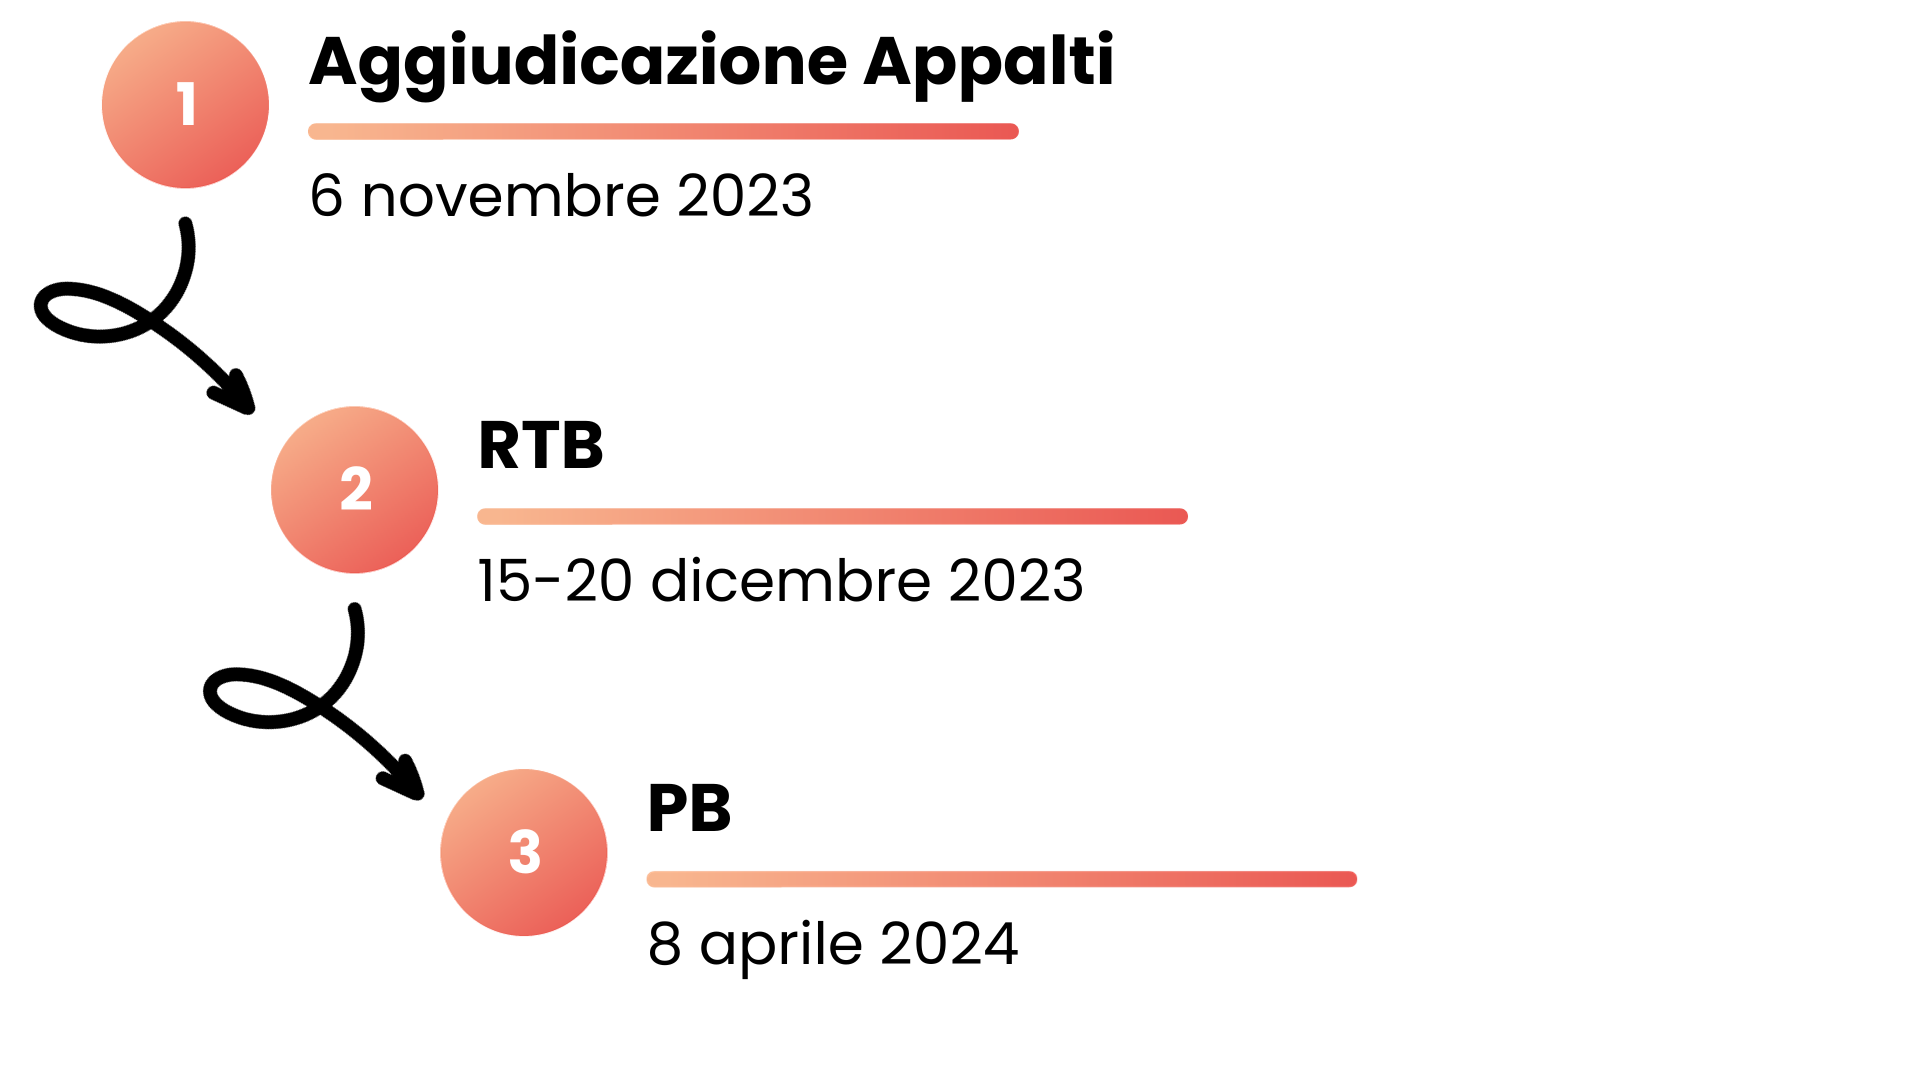
\includegraphics[width=10cm]{Calendario di massima - prima stesura.png}
        \caption{Grafico calendario - prima stesura}
    \end{figure}
\begin{comment}    
{\renewcommand{\arraystretch}{1.5}
\begin{table}[H]
\begin{tabularx}{\textwidth}{X|X}
\textbf{Revisione} & \textbf{Data} \\
\hline
Requirements \& Technology Baseline & \color{red} Periodo da $2023-12-15$ a $2023-12-20$ \color{black}\\
\hline
Product Baseline &  $2024-04-08$\\

\end{tabularx}
\caption{Tabella calendario di massima - prima stesura}
\end{table}}
\end{comment}


\section{Stima dei costi di realizzazione}
In questa sezione vengono riportate le stime dei costi e degli impegni orari alla luce di quanto analizzato nelle sezioni di \hyperref[section:Rischi]{\textbf{Rischi e mitigazione}} e \hyperref[section:Pianificazione]{\textbf{Pianificazione}}.

\subsection{Preventivo costi}
La stima dei costi di realizzazione non viene intaccata in maniera significativa dal cambiamento del calendario.

{\renewcommand{\arraystretch}{1.2}
\begin{table}[H]
\begin{tabularx}{\textwidth}{c|X|X|X|X|X|X|X}
        \textbf{Membri} & $\operatorname{\textbf{Re}}$ & $\mathrm{\textbf{Am}}$ & \textbf{An} & \textbf{Proj} & \textbf{Prgm} & \textbf{Ver} & \textbf{Tot} \\
        \hline Bresolin G. & 9 & 9 & 8 & 13 & 31 & 24 & 94 \\
        \hline Ciriolo I. & 11 & 11 & 10 & 16 & 27 & 19 & 94 \\
        \hline Campese M. & 10 & 10 & 8 & 15 & 26 & 25 & 94 \\
        \hline Dugo A. & 11 & 8 & 8 & 15 & 28 & 24 & 94 \\
        \hline Feltrin E. & 11 & 9 & 10 & 12 & 28 & 24 & 94 \\
        \hline Michelon R. & 9 & 8 & 10 & 13 & 30 & 24 & 94 \\
        \hline Orlandi G. & 9 & 8 & 9 & 14 & 26 & 28 & 94 
    \end{tabularx}
    \caption{Distribuzione ore - prima stesura}
    \end{table}

\subsubsubsection{Schema a torta di distribuzione ore ruoli} Di seguito viene illustrata la redistribuzione delle ore nei ruoli di progetto.
    \begin{figure}[H]
        \centering               
        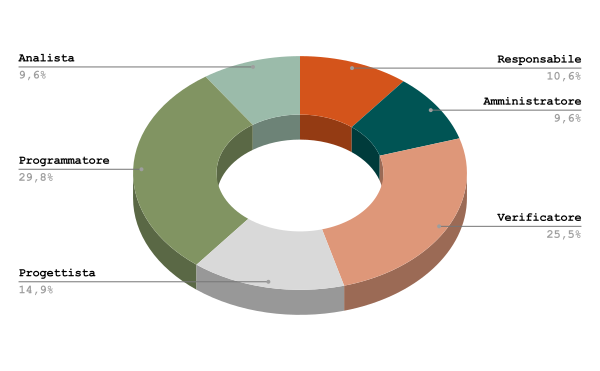
\includegraphics[width=14cm]{torta.png}
         \caption{Grafico ore percentuali - prima stesura}
    \end{figure}

{\renewcommand{\arraystretch}{1.2}
\begin{center}
\begin{table}[H]
    \begin{tabular}{l|c|c|c|c}
     \textbf{Ruoli} & \textbf{Costo Orario} & \textbf{Ore per Ruolo} & \quantities{\textbf{Ore Medie per}\\\textbf{Membro}} & \textbf{Percentuale Ore} \\
    \hline Responsabile & 30,00\texteuro & 70 & 10 & 10.6\% \\
    \hline Amministratore & 20,00\texteuro & 63 & 9 & 9.6\%\% \\
    \hline Verificatore & 15,00\texteuro & 168 & 24 & 25.5\% \\
    \hline Progettista & 25,00\texteuro & 98 & 14 & 14.9\%\% \\
    \hline Programmatore & 15,00\texteuro & 196 & 28 & 29.8\% \\
    \hline Analista & 25,00\texteuro & 63 & 9 & 9.6\%\\
    \hline  & \textbf{Totale Costo} & \textbf{Totale Ore} & \quantities{\textbf{Totale Ore per}\\\textbf{Membro}}\\
    \hline  & \cellcolor{primarycolor} 12845,00\texteuro & \cellcolor{primarycolor}658 &\cellcolor{primarycolor} 94 \\
    \end{tabular}
    \caption{Costo totale - prima stesura}
    \end{table}
\end{center}

%    PIANIFICAZIONE
\section{Pianificazione e modello di sviluppo}
\label{section:Pianificazione}

Il team decide di adottare il modello di sviluppo \textit{Agile} 
promuovendo un approccio incrementale al lavoro; questo consentirà di suddividere il progetto in compiti più gestibili, ovvero \textit{sprint}, ciascuno dei quali produrrà risultati funzionanti. Questo consente al team di progetto di reagire ai cambiamenti in modo più efficace.
Il team definisce in seguito una pianificazione generale che verrà approfondita prima di ogni sprint.
I periodi individuati sono \textit{sprint} di 14 giorni con conseguente rotazione dei ruoli assunti dai componenti del gruppo.\\
Questo tipo di pianificazione permette di avere un orizzonte temporale limitato, sebbene vi sia una pianificazione dell'intero periodo del progetto; ciò aiuta nel caso in cui vengano riscontrate difficoltà che causano danni ad attività che dipendono le une dalle altre. In questi casi è quindi possibile contenere i danni e riorganizzare le attività nel periodo successivo.

\subsection{Requirements and Technology Baseline}
Questo periodo antecedente la revisione RTB di progetto si focalizza sulla preparazione dei documenti (Analisi dei requisiti, Piano di progetto, Piano di qualifica, ampliamento Norme di progetto) e sulla creazione del \textit{Proof of Concept} per il progetto.
%\vspace{2em}
\subsubsection{Periodo 1: da 2023-11-07 a 2023-11-21}
Questo primo periodo segue l'assegnazione dei capitolati e viene utilizzato principalmente per configurare l'ambiente di lavoro, le norme e per studiare i casi d'uso e perseguire l'analisi dei requisiti del progetto. Infine lo \textit{sprint} si concentra sullo studio e selezione di tecnologie utili allo sviluppo del progetto.
\subsubsubsection{Obiettivi}
\begin{itemize}
    \item Stesura e ampliamento delle Norme di progetto;
    \item Prima stesura Analisi dei requisiti;
    \item Automazione versionamento;
    \item Manutenzione ambiente di lavoro;
    \item Software selection;
    \item Verbali delle riunioni.
        
\end{itemize}
%\paragraph{Diagramma di Gantt}
\vspace{1em}

 \begin{figure}[H]
        \centering        
        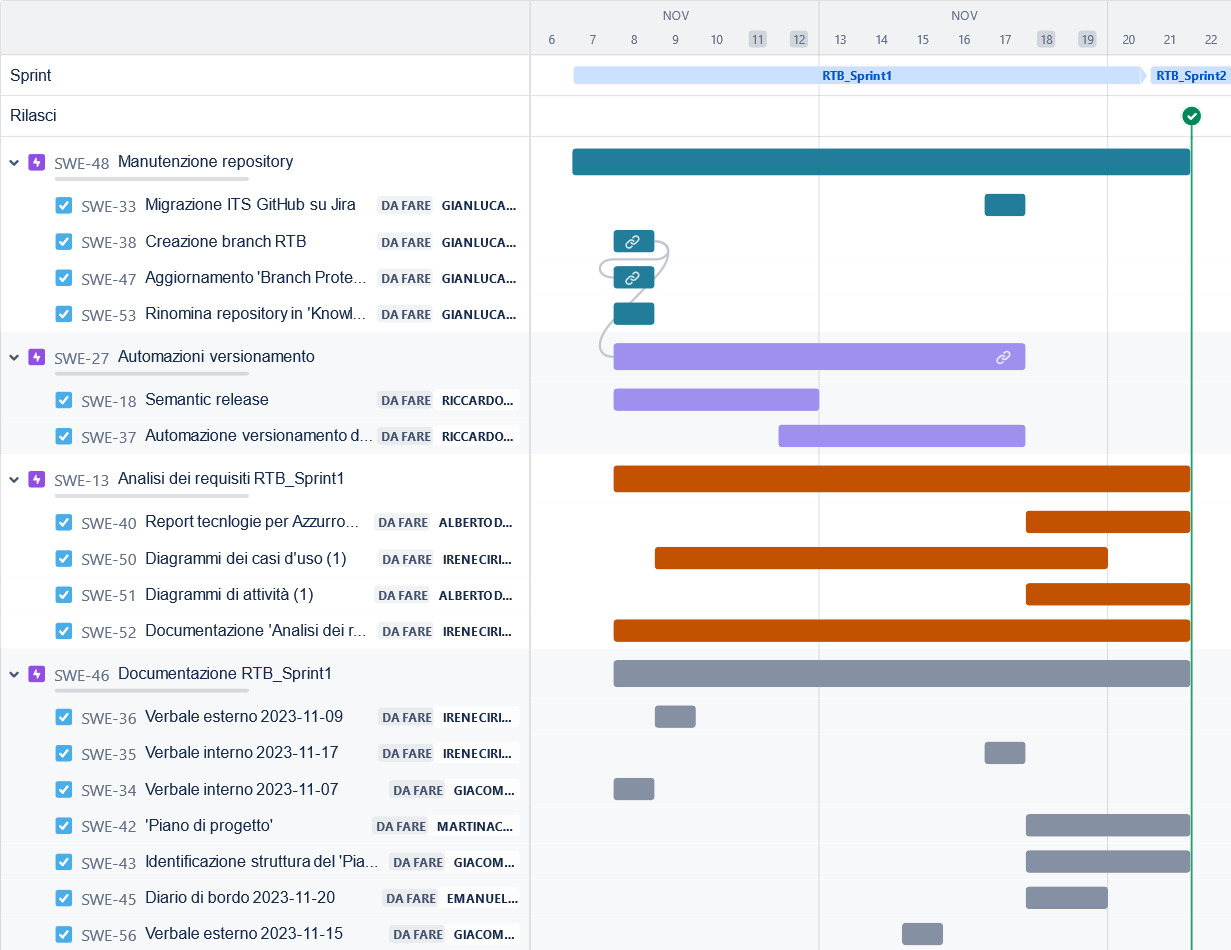
\includegraphics[width=15.5cm]{ganttPeriodo1.png}
        \caption{Diagramma di Gantt Periodo 1 }
    \end{figure}

%\vspace{2em}
\subsubsection{Periodo 2: da 2023-11-21 a 2023-12-05}
In questo periodo le ore di lavoro sono concentrate nella creazione di un PoC richiesto dall'azienda e nell'ampliamento e miglioramento della documentazione necessaria per guidare l'avanzamento del progetto.
\subsubsubsection{Obiettivi}
\begin{itemize}
    \item Progettazione PoC;
    \item Codifica PoC;
    \item Prosecuzione stesura Analisi dei requisiti;
    \item Migliorie Norme di progetto e Piano di progetto;
    \item Stesura correttiva Piano di qualifica;
    \item Verbali delle riunioni.
  
\end{itemize}
%\paragraph{Diagramma di Gantt}
\vspace{1em}

 \begin{figure}[H]
        \centering        
        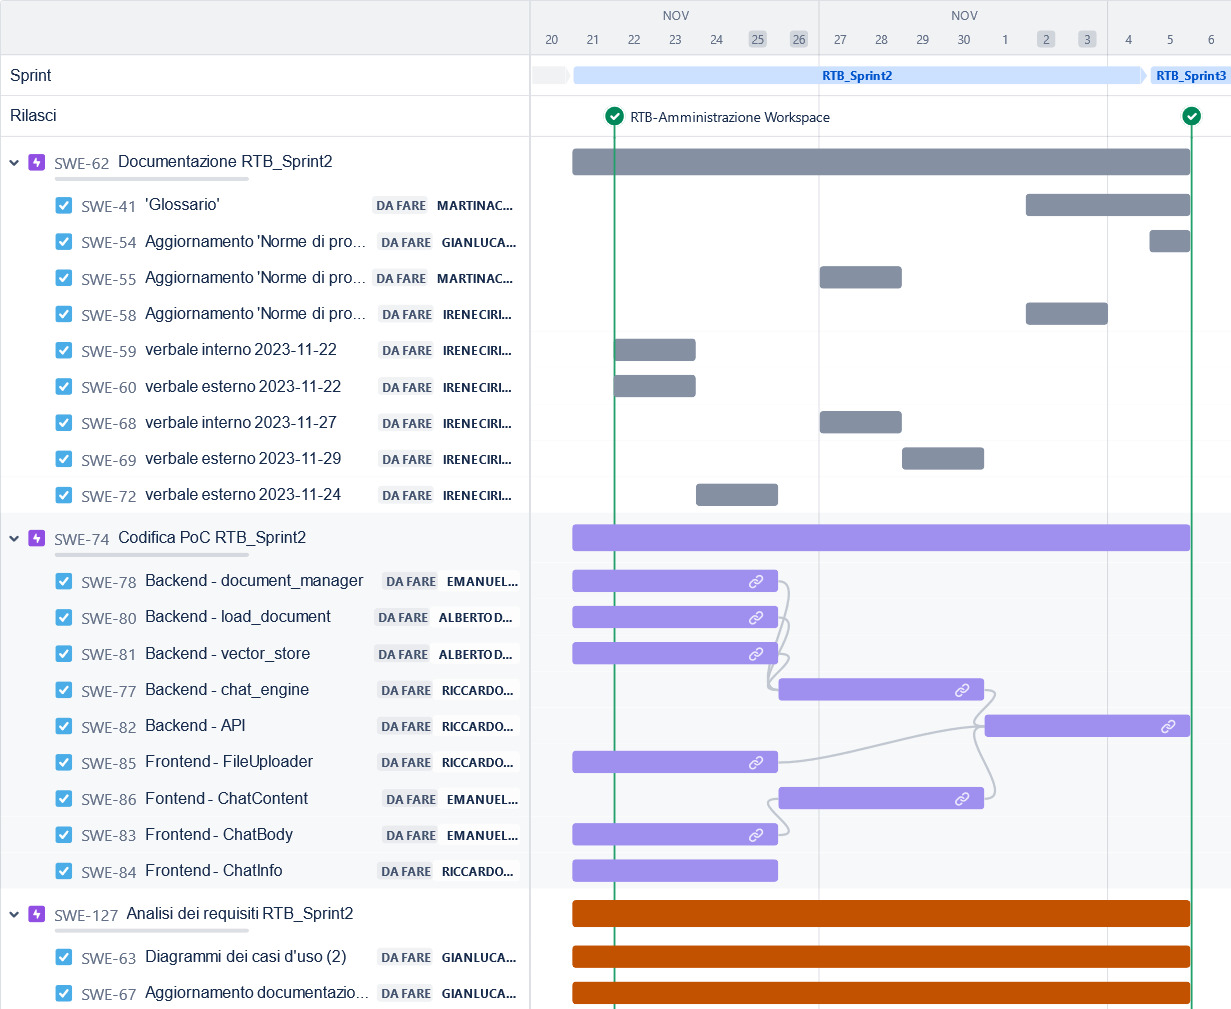
\includegraphics[width=15.5cm]{ganttPeriodo2.png}
        \caption{Diagramma di Gantt Periodo 2 }
    \end{figure}

\subsubsection{Periodo 3: da 2023-12-05 a 2023-12-19}
\subsubsubsection{Obiettivi}
\begin{itemize}
    \item Refactoring codice PoC;
    \item Refactoring architettura PoC;
    \item Correzione e conclusione stesura Analisi dei requisiti;
    \item Migliorie Norme di progetto e ampliamento Piano di progetto alla luce del Piano di Qualifica;
    \item Ampliamento sostanziale del Piano di qualifica;
    \item Verbali delle riunioni.
\end{itemize}
\begin{figure}[H]
    \centering        
    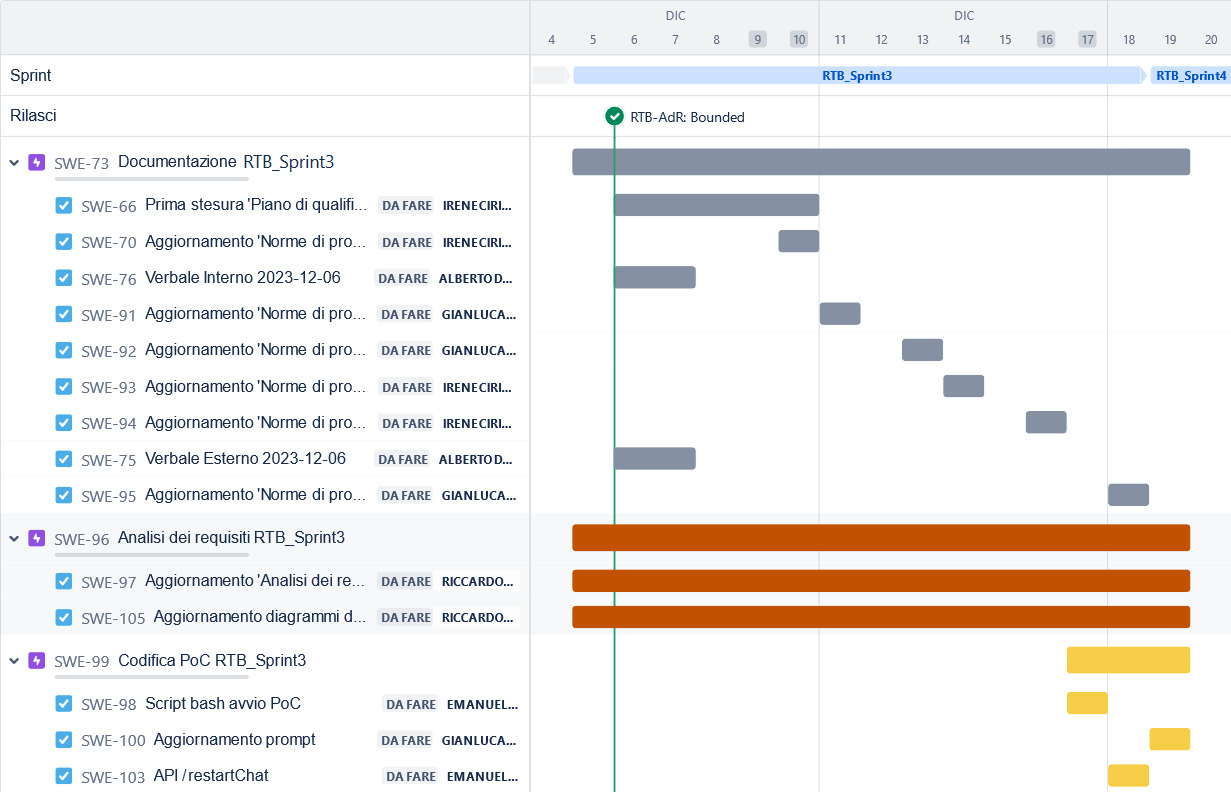
\includegraphics[width=15.5cm]{ganttPeriodo3.png}
    \caption{Diagramma di Gantt Periodo 3 }
\end{figure}

\subsubsection{Periodo 4: da 2023-12-19 a 2024-01-02}
\subsubsubsection{Obiettivi}
\begin{itemize}
    \item Progettazione con Azzurro Digitale;
    \item Piano di qualifica;
    \item Aggiornamento Piano di progetto.
    \item Verbali delle riunioni.
\end{itemize}
\subsection{Product Baseline}

\subsubsection{Periodo 5: da 2024-01-02 a 2024-01-16}
\subsubsubsection{Obiettivi}
\begin{itemize}
    \item Progettazione con Azzurro Digitale;
    \item Piano di qualifica;
    \item Aggiornamento Piano di progetto.
    \item Verbali delle riunioni.
\end{itemize}

\subsubsection{Periodo 6: da 2024-01-16 a 2024-01-30}
%
\subsubsubsection{Obiettivi}
\begin{itemize}
    \item Progettazione con Azzurro Digitale;
    \item Inizio programmazione;
    \item Primi test;
    \item Piano di qualifica;
    \item Aggiornamento Piano di progetto.
    \item Verbali delle riunioni.
\end{itemize}

\subsubsection{Periodo 7: da 2024-01-30 a 2024-02-13}
%
\subsubsubsection{Obiettivi}
\begin{itemize}
    \item Progettazione di dettaglio;
    \item Programmazione;
    \item Test di unità;
    \item Documentazione relativa al codice;
    \item Aggiornamento Piano di qualifica;
    \item Aggiornamento Piano di progetto.
    \item Verbali delle riunioni.
\end{itemize}

\subsubsection{Periodo 8: da 2024-02-13 a 2024-02-27}
%
\subsubsubsection{Obiettivi}
\begin{itemize}
    \item Progettazione di dettaglio;
    \item Programmazione;
    \item Test di unità e di integrazione;
    \item Documentazione relativa al codice;
    \item Aggiornamento Piano di qualifica;
    \item Aggiornamento Piano di progetto.
    \item Verbali delle riunioni.
\end{itemize}

\subsubsection{Periodo 9: da 2024-02-27 a 2024-03-12}
%
\subsubsubsection{Obiettivi}
\begin{itemize}
    \item Programmazione;
    \item Test di unità e di integrazione;
    \item Documentazione relativa al codice;
    \item Aggiornamento Piano di qualifica;
    \item Aggiornamento Piano di progetto.
    \item Verbali delle riunioni.
\end{itemize}

\subsubsection{Periodo 10: da 2024-03-12 a 2024-03-26}
%
\subsubsubsection{Obiettivi}
\begin{itemize}
    \item Programmazione;
    \item Test di integrazione;
    \item Test di sistema;
    \item Documentazione relativa al codice;
    \item Aggiornamento Piano di qualifica;
    \item Aggiornamento Piano di progetto;
    \item Verbali delle riunioni.
\end{itemize}
\subsubsection{Periodo 11: da 2024-03-26 a 2024-04-08}
%
\subsubsubsection{Obiettivi}
\begin{itemize}
    \item Conclusione Programmazione;
    \item Documentazione relativa al codice;
    \item Aggiornamento Piano di qualifica;
    \item Aggiornamento Piano di progetto;
    \item Verbali delle riunioni.
\end{itemize}


\newpage
% PREVENTIVO

\section{Preventivo}
Ogni membro del team mette a disposizione le sue conoscenze e le 94 ore produttive ciascuno, divise nei vari ruoli. Il preventivo è stato calcolato in base al costo orario di ciascun componente, e in base alla nostra previsione di attività da svolgere in ogni sprint. Di seguito, vengono dettagliati gli aspetti di ciascun incremento e il relativo costo. La distribuzione dei ruoli tra i membri è stata equa, offrendo a ognuno l'opportunità di sperimentare diverse mansioni. Abbreviazioni specifiche sono utilizzate nelle tabelle per brevità:
\begin{itemize}
    \item Re: Responsabile;
    \item Am: Amministratore;
    \item An: Analista;
    \item Proj: Progettista;
    \item Prgm: Programmatore;
    \item Ver: Verificatore.
\end{itemize}
Nelle tabelle sottostanti relative al preventivo è possibile trovare una cella colorata per ogni membro del team, la quale si riferisce al ruolo che il membro stesso assumerà.
% SPRINT 1 PREVENTIVO
\subsubsection{Sprint 1: da 2023-11-07 a 2023-11-21}
Di seguito, la distribuzione delle ore del primo sprint; ogni componente del gruppo rivestirà i ruoli come segue:
\begin{table}[H]
\begin{tabularx}{\textwidth}{c|X|X|X|X|X|X|X}
        \textbf{Membri} & $\operatorname{\textbf{Re}}$ & $\mathrm{\textbf{Am}}$ & \textbf{An} & \textbf{Proj} & \textbf{Prgm} & \textbf{Ver} & \textbf{Totale} \\
        \hline Bresolin G. & 0 & \cellcolor{primarycolor}4 & 0 & 0 & 0 & 0 & 4 \\
        \hline Ciriolo I.  & 0 & 0 & \cellcolor{primarycolor}6 & 0 & 0 & 1 & 7 \\
        \hline Campese M.  & 0 & 0 & 2 & 0 & 0 & \cellcolor{primarycolor}8 & 10 \\
        \hline Dugo A.     & 0 & \cellcolor{primarycolor}4 & 0 & 0 & 0 & 0 & 4 \\
        \hline Feltrin E.  & \cellcolor{primarycolor}8 & 1 & 0 & 0 & 0 & 0 & 9 \\
        \hline Michelon R. & 0 & \cellcolor{primarycolor}6 & 0 & 0 & 0 & 0 & 6 \\
        \hline Orlandi G.  & 0 & 0 & \cellcolor{primarycolor}3 & 0 & 0 & 1 & 4 \\
        \hline
        \textbf{Totale ruolo} & 8 & 15 & 11 & 0 & 0 & 10 & 44 
    \end{tabularx}
    \caption{Preventivo ore - Sprint 1}
    \end{table}

La tabella è riassunta dal seguente istogramma:
 \begin{figure}[H]
        \centering        
        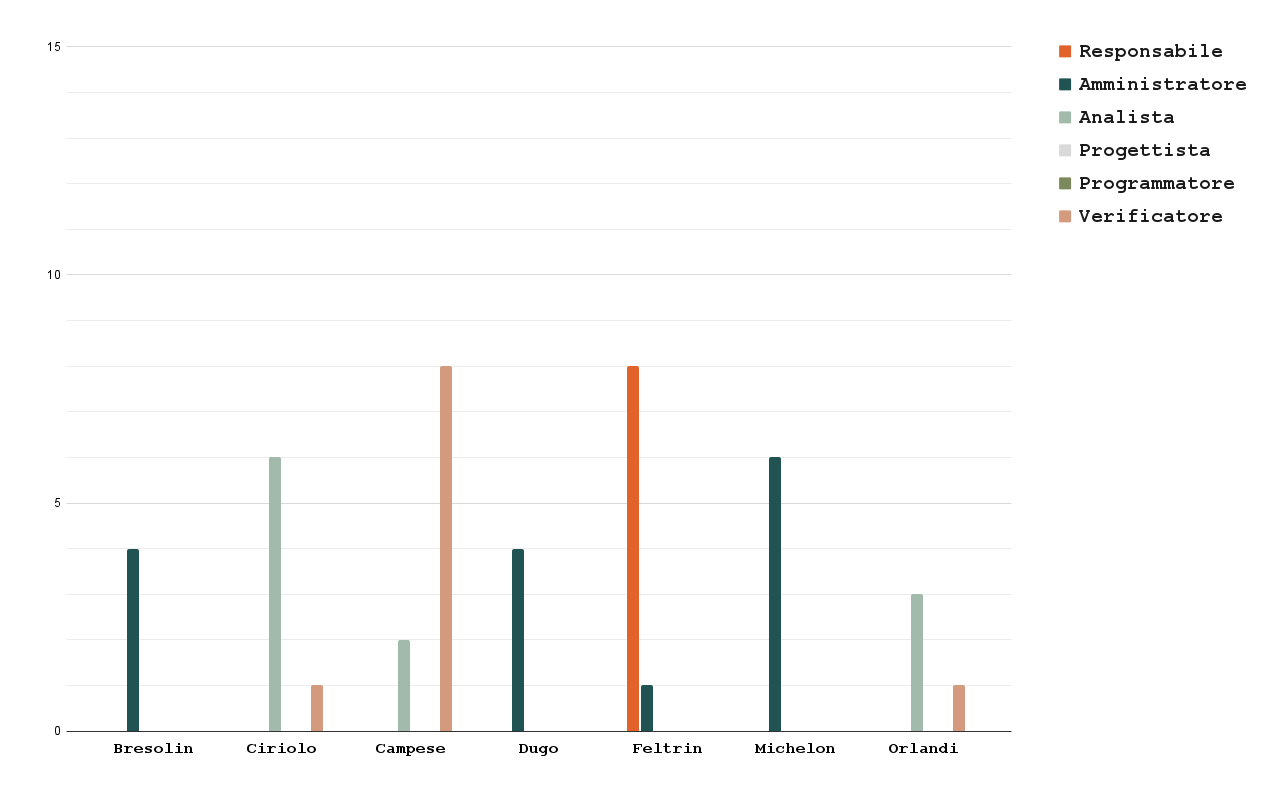
\includegraphics[width=15.5cm]{istogrammi/istogramma_1_periodo.png}
        \caption{Sprint 1 - Istogramma della ripartizione oraria dei ruoli. }
    \end{figure}
 
In questo incremento, il costo per ogni ruolo sarà come da tabella:
{\renewcommand{\arraystretch}{1.5}
\begin{table}[H]
\centering
\begin{tabularx}{0.42\textwidth}{c|c|c}

\textbf{Ruolo} & \textbf{Ore} & \textbf{Costo}\\
\hline
\textbf{Responsabile} & 8 & 240,00\texteuro\\
\hline
\textbf{Amministratore} & 15 & 300,00\texteuro \\
\hline
\textbf{Analista} & 11 & 275,00\texteuro \\
\hline
\textbf{Progettista} & 0 & 0\texteuro\\
\hline
\textbf{Programmatore} & 0 & 0\texteuro \\ 
\hline
\textbf{Verificatore} & 10 & 150,00\texteuro \\ 
\hline
\rowcolor{primarycolor}
\textbf{Totale} & 44 & 965,00\texteuro \\
\end{tabularx}
%}
\caption{Preventivo costi - Sprint 1}
\end{table}

La tabella è riassunta dal seguente aereogramma:
 \begin{figure}[H]
        \centering        
        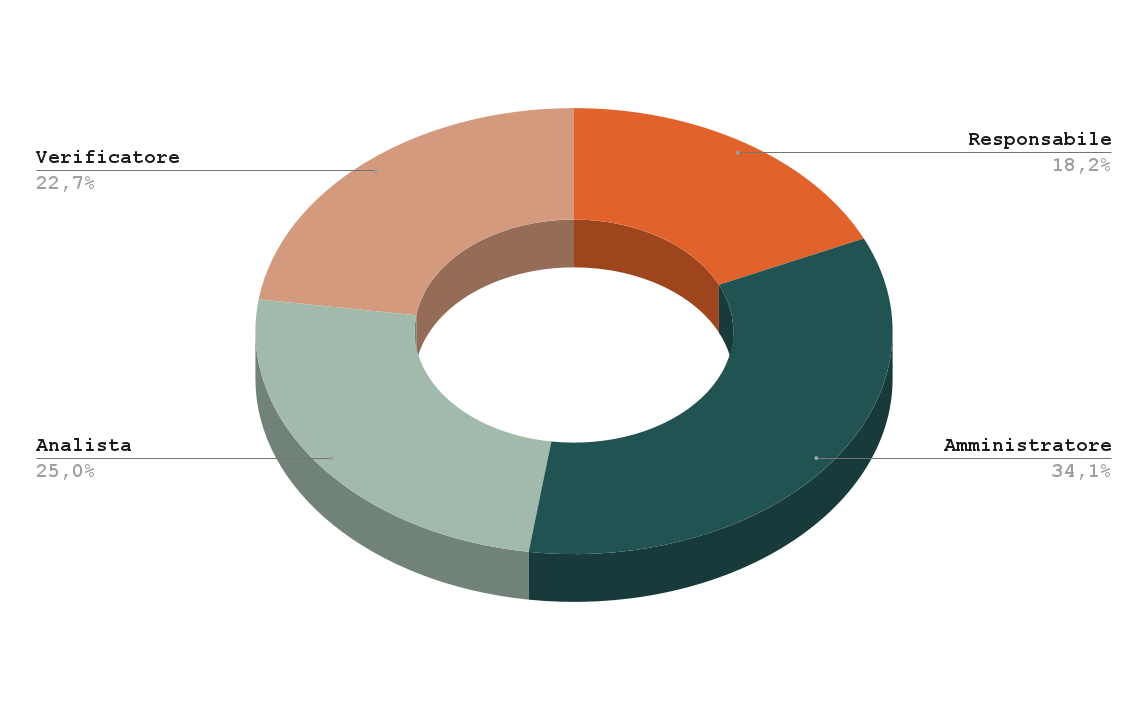
\includegraphics[width=15.5cm]{aereogrammi/areogramma_1_periodo.png}
        \caption{Sprint 1 - Areogramma della ripartizione oraria dei ruoli. }
    \end{figure}


%SPRINT 2 PREVENTIVO
\subsubsection{Sprint 2: da 2023-11-21 a 2023-12-05 }

Di seguito, la distribuzione delle ore del secondo sprint; ogni componente del gruppo rivestirà i ruoli come segue:

\begin{table}[H]
\begin{tabularx}{\textwidth}{c|X|X|X|X|X|X|X}
        \textbf{Membri} & $\operatorname{\textbf{Re}}$ & $\mathrm{\textbf{Am}}$ & \textbf{An} & \textbf{Proj} & \textbf{Prgm} & \textbf{Ver} & \textbf{Totale} \\
        \hline Bresolin G. & 0 & 1 & \cellcolor{primarycolor}6 & 0 & 0 & 0 & 7 \\
        \hline Ciriolo I.  & \cellcolor{primarycolor}7 & 0 & 0 & 0 & 0 & 1 & 8 \\
        \hline Campese M.  & 0 & \cellcolor{primarycolor}5 & 2 & 0 & 0 & 1,5 & 8,5 \\
        \hline Dugo A.     & 0 & 0 & 2 & \cellcolor{primarycolor}2 & 9 & 0 & 13 \\
        \hline Feltrin E.  & 0 & 0 & 0 & 0 & \cellcolor{primarycolor}11 & 0 & 11 \\
        \hline Michelon R. & 0 & 0 & 2 & 1 & \cellcolor{primarycolor}13 & 0 & 16 \\
        \hline Orlandi G.  & 0 & 0 & 0 & 0 & 0 & \cellcolor{primarycolor}7 & 7 \\
        \hline
        \textbf{Totale ruolo} & 7 & 6 & 12 & 3 & 33 & 9,5 & 70,5 
    \end{tabularx}
    \caption{Preventivo ore - Sprint 2}
    \end{table}

La tabella è riassunta dal seguente istogramma:
 \begin{figure}[H]
        \centering        
        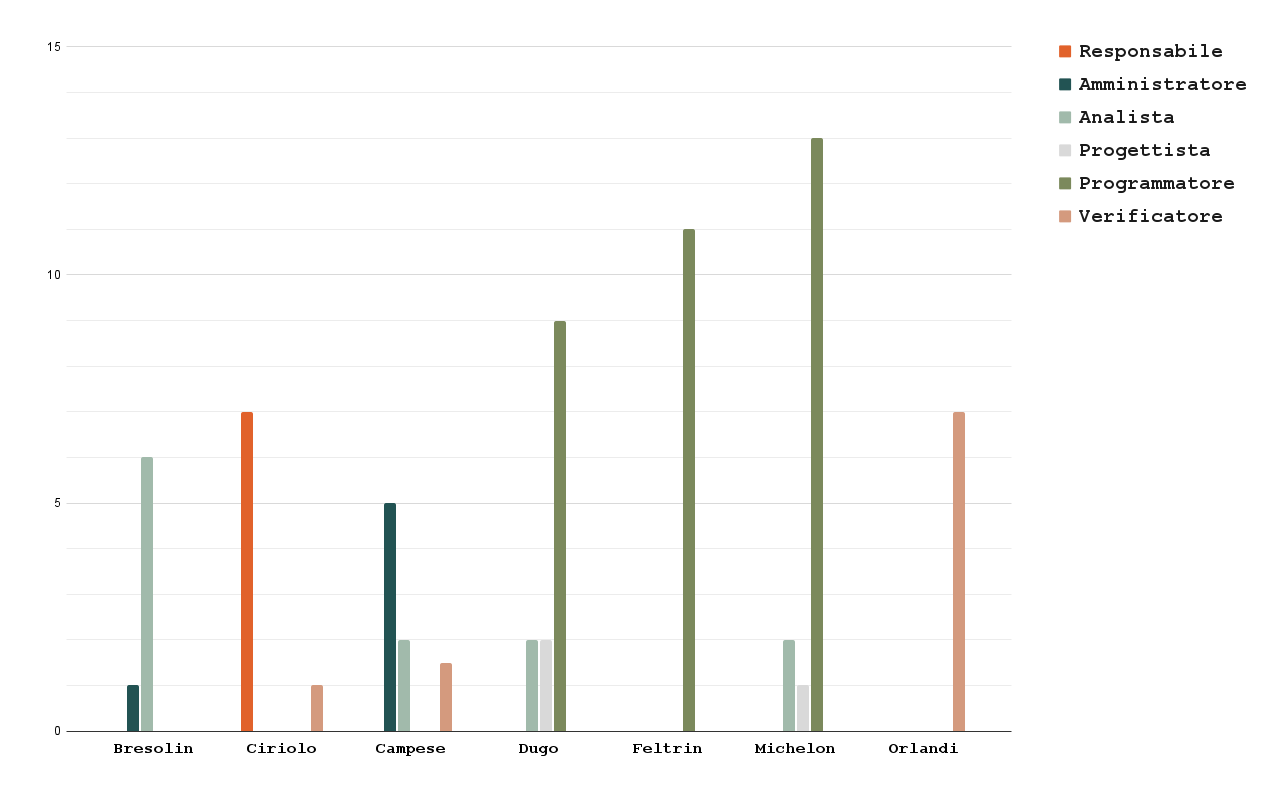
\includegraphics[width=15.5cm]{istogrammi/istogramma_2_periodo.png}
        \caption{Sprint 2 - Istogramma della ripartizione oraria dei ruoli. }
    \end{figure}
 
In questo incremento, il costo per ogni ruolo sarà come da tabella:
{\renewcommand{\arraystretch}{1.5}
\begin{table}[H]
\centering
\begin{tabularx}{0.42\textwidth}{c|c|c}

\textbf{Ruolo} & \textbf{Ore} & \textbf{Costo}\\
\hline
\textbf{Responsabile} & 7 & 210,00\texteuro\\
\hline
\textbf{Amministratore} & 6 & 120,00\texteuro \\
\hline
\textbf{Analista} & 12 & 300,00\texteuro \\
\hline
\textbf{Progettista} & 3 & 75,00\texteuro\\
\hline
\textbf{Programmatore} & 33 & 495,00\texteuro \\ 
\hline
\textbf{Verificatore} & 9,5 & 142,50\texteuro \\ 
\hline
\rowcolor{primarycolor}
\textbf{Totale} & 70,5 & 1342,50\texteuro \\
\end{tabularx}
%}
\caption{Preventivo costi - Sprint 2}
\end{table}


La tabella è riassunta dal seguente aereogramma:
 \begin{figure}[H]
        \centering        
        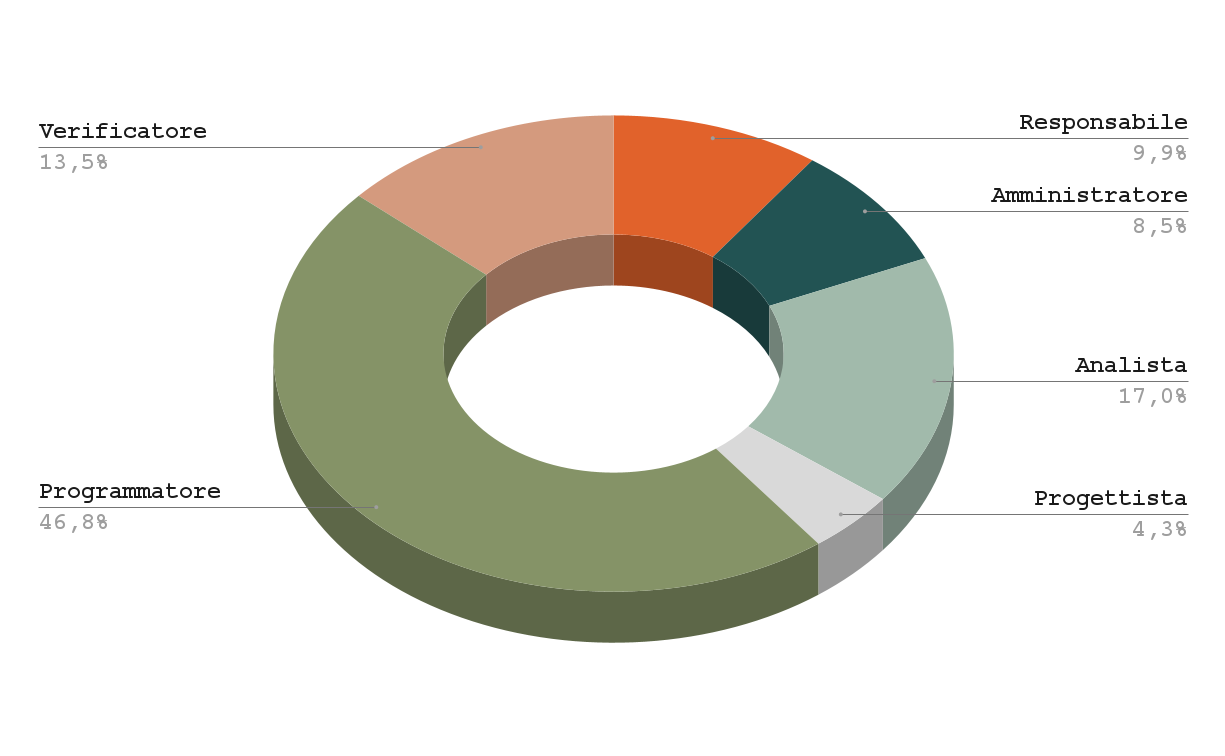
\includegraphics[width=15.5cm]{aereogrammi/areogramma_2_periodo.png}
        \caption{Sprint 2 - Areogramma della ripartizione oraria dei ruoli. }
    \end{figure}





\subsubsection{Sprint 3: da 2023-12-05 a 2023-12-19}
Di seguito, la distribuzione delle ore del terzo sprint; ogni componente del gruppo rivestirà i ruoli come segue:
\begin{table}[H]
\begin{tabularx}{\textwidth}{c|X|X|X|X|X|X|X}
        \textbf{Membri} & $\operatorname{\textbf{Re}}$ & $\mathrm{\textbf{Am}}$ & \textbf{An} & \textbf{Proj} & \textbf{Prgm} & \textbf{Ver} & \textbf{Totale} \\
        \hline Bresolin G. & 0 & 0 & 2 & 1 & 0 & \cellcolor{primarycolor}7 & 10 \\
        \hline Ciriolo I.  & 0 & \cellcolor{primarycolor}4 & 1 & 0 & 0 & 3 & 7 \\
        \hline Campese M.  & 0 & 0 & \cellcolor{primarycolor}2 & 0 & 0 & 4 & 6 \\
        \hline Dugo A.     & \cellcolor{primarycolor}6 & 0 & 2 & 0 & 0 & 0 & 8 \\
        \hline Feltrin E.  & 0 & 0 & \cellcolor{primarycolor}8 & 0 & 0 & 0 & 8 \\
        \hline Michelon R. & 0 & 0 & \cellcolor{primarycolor}7 & 0 & 0 & 0 & 7 \\
        \hline Orlandi G.  & 0 & 0 & 3 & 0 & \cellcolor{primarycolor}4 & 0 & 7 \\
        \hline
        \textbf{Totale ruolo} & 6 & 4 & 25 & 1 & 4 & 14 & 54 
    \end{tabularx}
    \caption{Preventivo ore - Sprint 3}
    \end{table}

La tabella è riassunta dal seguente istogramma:
 \begin{figure}[H]
        \centering        
        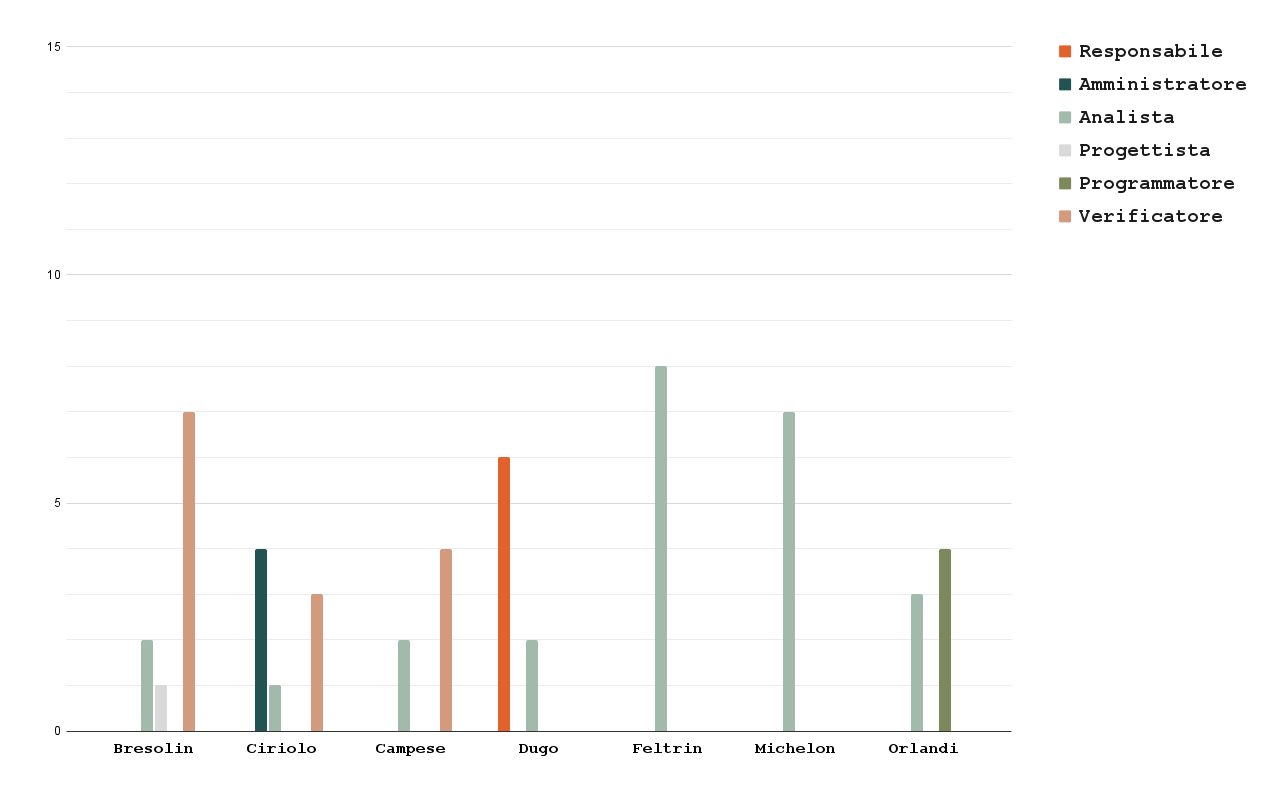
\includegraphics[width=15.5cm]{istogrammi/istogramma_3_periodo.png}
        \caption{Sprint 3 - Istogramma della ripartizione oraria dei ruoli. }
    \end{figure}

In questo incremento, il costo per ogni ruolo sarà come da tabella:
{\renewcommand{\arraystretch}{1.5}
\begin{table}[H]
\centering
\begin{tabularx}{0.42\textwidth}{c|c|c}

\textbf{Ruolo} & \textbf{Ore} & \textbf{Costo}\\
\hline
\textbf{Responsabile} & 6 & 180,00\texteuro\\
\hline
\textbf{Amministratore} & 4 & 80,00\texteuro \\
\hline
\textbf{Analista} & 25 & 625,00\texteuro \\
\hline
\textbf{Progettista} & 1 & 25,00\texteuro\\
\hline
\textbf{Programmatore} & 4 & 60,00 \texteuro \\ 
\hline
\textbf{Verificatore} & 14 & 210,00\texteuro \\ 
\hline
\rowcolor{primarycolor}
\textbf{Totale} & 53 & 1180,00\texteuro \\
\end{tabularx}
%}
\caption{Preventivo costi - Sprint 3}
\end{table}


La tabella è riassunta dal seguente aereogramma:
 \begin{figure}[H]
        \centering        
        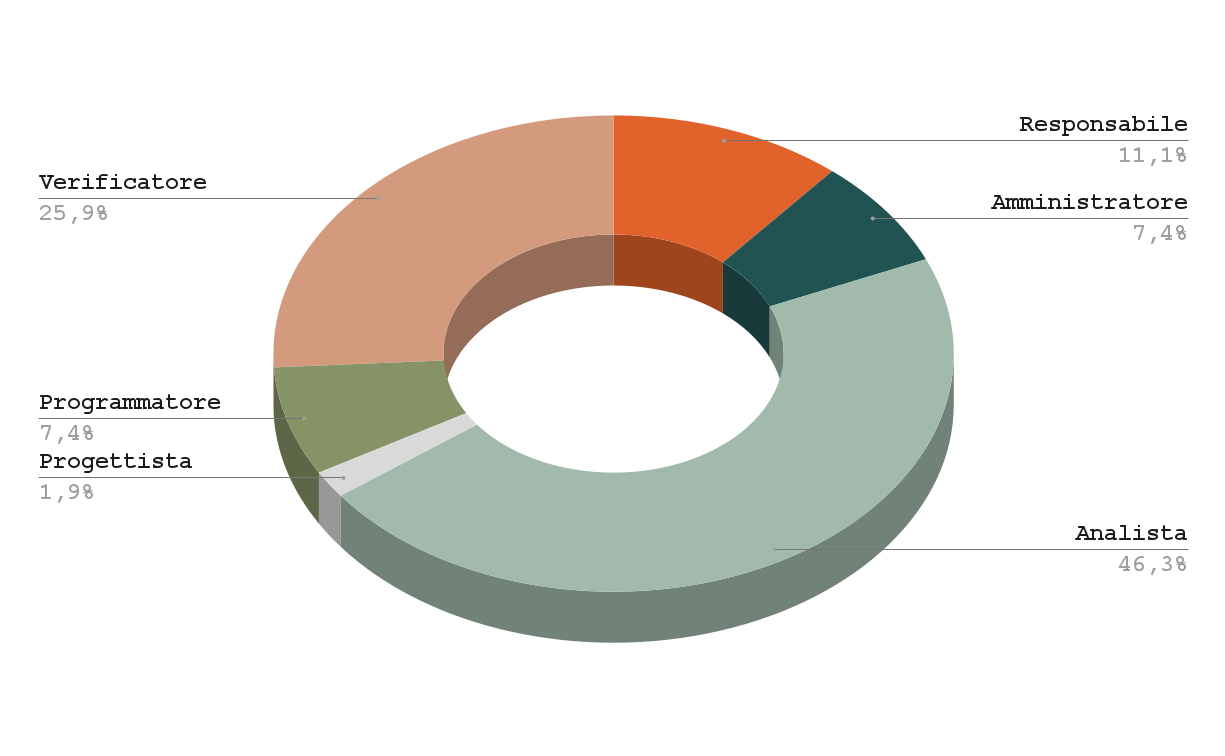
\includegraphics[width=15.5cm]{aereogrammi/areogramma_3_periodo.png}
        \caption{Sprint 3 - Areogramma della ripartizione oraria dei ruoli. }
    \end{figure}



%   PERIODO 4

\subsubsection{Sprint 4: da 2023-12-19 a 2024-01-02}
Di seguito, la distribuzione delle ore del quarto sprint; ogni componente del gruppo rivestirà i ruoli come segue:
\begin{table}[H]
\begin{tabularx}{\textwidth}{c|X|X|X|X|X|X|X}
        \textbf{Membri} & $\operatorname{\textbf{Re}}$ & $\mathrm{\textbf{Am}}$ & \textbf{An} & \textbf{Proj} & \textbf{Prgm} & \textbf{Ver} & \textbf{Totale} \\
        \hline Bresolin G. & 0 & 0 & 0 & 0 & \cellcolor{primarycolor}7 & 0 & 7 \\
        \hline Ciriolo I.  & 0 & 0 & 0 & \cellcolor{primarycolor}8 & 0 & 0 & 8 \\
        \hline Campese M.  & \cellcolor{primarycolor}6 & 0 & 2 & 3 & 0 & 0 & 11 \\
        \hline Dugo A.     & 0 & 0 & 1 & \cellcolor{primarycolor}10 & 0 & 0 & 11 \\
        \hline Feltrin E.  & 0 & \cellcolor{primarycolor}4 & 0 & 0 & 3 & 1 & 8 \\
        \hline Michelon R. & 0 & 0 & 0 & \cellcolor{primarycolor}5 & 0 & 0 & 5 \\
        \hline Orlandi G.  & 0 & 1 & 3 & 0 & 0 & \cellcolor{primarycolor}7 & 11 \\
        \hline
        \textbf{Totale ruolo} & 6 & 5 & 6 & 26 & 10 & 8 & 61 
    \end{tabularx}
    \caption{Preventivo ore - Sprint 4}
    \end{table}

La tabella è riassunta dal seguente istogramma:
 \begin{figure}[H]
        \centering        
        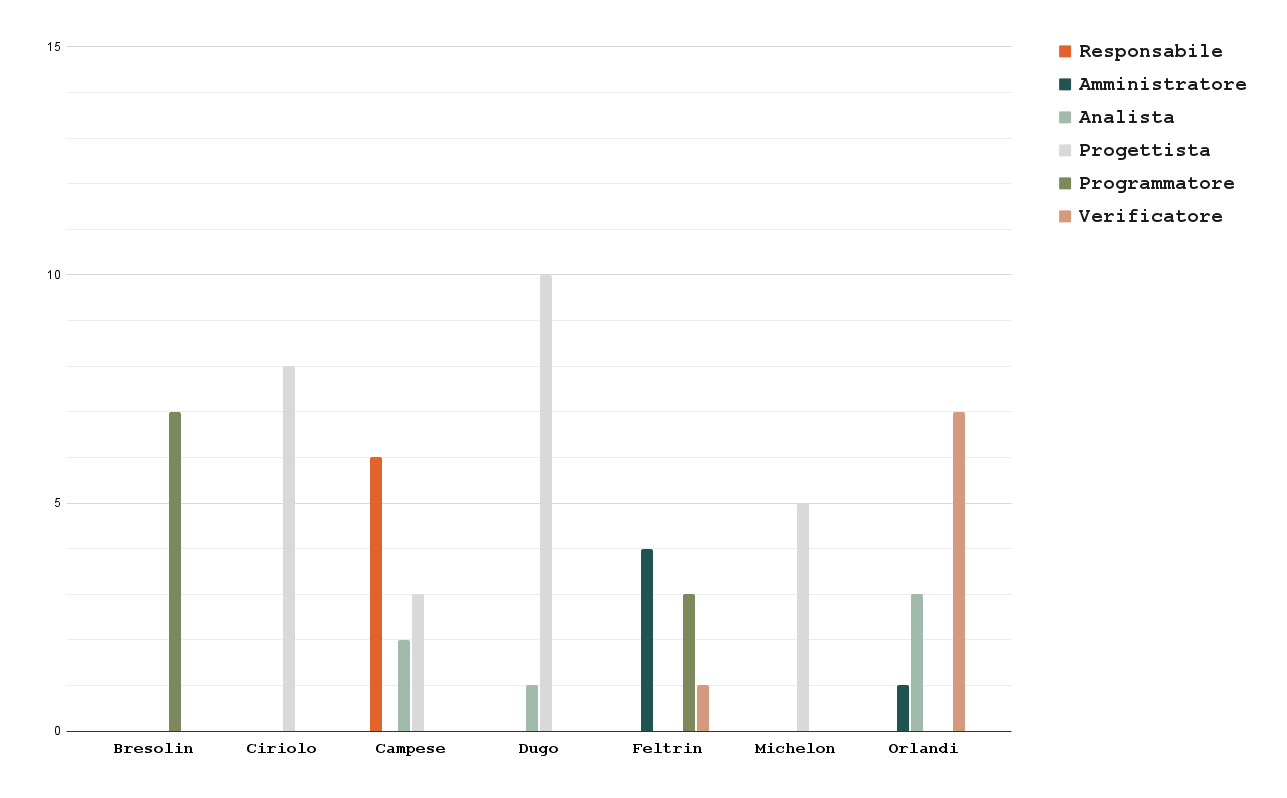
\includegraphics[width=15.5cm]{istogrammi/istogramma_4_periodo.png}
        \caption{Sprint 4 - Istogramma della ripartizione oraria dei ruoli. }
    \end{figure}

In questo incremento, il costo per ogni ruolo sarà come da tabella:
{\renewcommand{\arraystretch}{1.5}
\begin{table}[H]
\centering
\begin{tabularx}{0.42\textwidth}{c|c|c}

\textbf{Ruolo} & \textbf{Ore} & \textbf{Costo}\\
\hline
\textbf{Responsabile} & 6 & 180,00\texteuro\\
\hline
\textbf{Amministratore} & 5 & 100,00\texteuro \\
\hline
\textbf{Analista} & 6 & 150,00\texteuro \\
\hline
\textbf{Progettista} & 26 & 650,00\texteuro\\
\hline
\textbf{Programmatore} & 10 & 150,00 \texteuro \\ 
\hline
\textbf{Verificatore} & 8 & 120,00\texteuro \\ 
\hline
\rowcolor{primarycolor}
\textbf{Totale} & 61 & 1350,00\texteuro \\
\end{tabularx}
%}
\caption{Preventivo costi - Sprint 4}
\end{table}

La tabella è riassunta dal seguente aereogramma:
 \begin{figure}[H]
        \centering        
        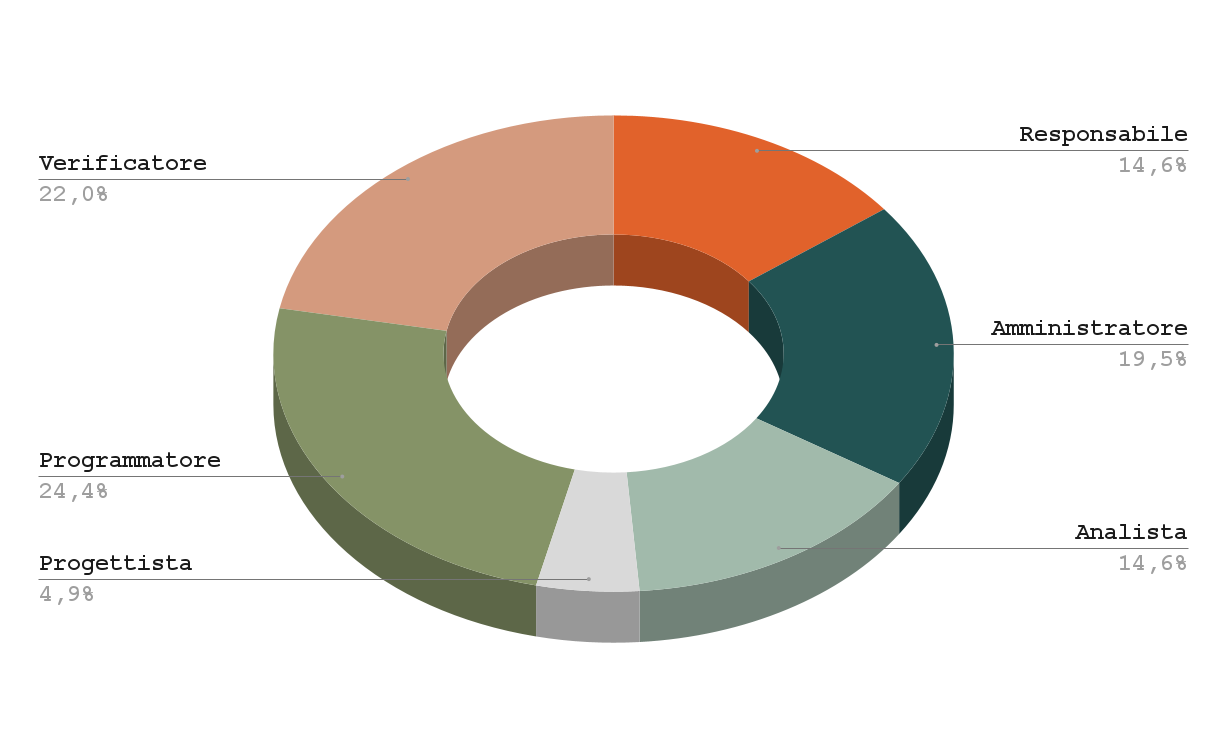
\includegraphics[width=15.5cm]{aereogrammi/areogramma_4_periodo.png}
        \caption{Sprint 4 - Areogramma della ripartizione oraria dei ruoli. }
    \end{figure}





%   PERIODO 5


\subsubsection{Sprint 5: da 2023-01-02 a 2024-01-16}
Di seguito, la distribuzione delle ore del quinto sprint; ogni componente del gruppo rivestirà i ruoli come segue:
\begin{table}[H]
\begin{tabularx}{\textwidth}{c|X|X|X|X|X|X|X}
        \textbf{Membri} & $\operatorname{\textbf{Re}}$ & $\mathrm{\textbf{Am}}$ & \textbf{An} & \textbf{Proj} & \textbf{Prgm} & \textbf{Ver} & \textbf{Totale} \\
        \hline Bresolin G. & 0 & 0 & 0 & \cellcolor{primarycolor}10 & 0 & 0 & 10 \\
        \hline Ciriolo I.  & 0 & 0 & 3 & \cellcolor{primarycolor}5 & 0 & 4 & 12 \\
        \hline Campese M.  & 0 & 0 & 0 & \cellcolor{primarycolor}5 & 6 & 0 & 11 \\
        \hline Dugo A.     & 0 & 0 & 0 & 0 & \cellcolor{primarycolor}10 & 0 & 10 \\
        \hline Feltrin E.  & 0 & 0 & 0 & 4 & 0 & \cellcolor{primarycolor}5 & 9 \\
        \hline Michelon R. & \cellcolor{primarycolor}6 & 0 & 0 & 5 & 0 & 0 & 11 \\
        \hline Orlandi G.  & 0 & \cellcolor{primarycolor}4 & 0 & 1 & 3 & 0 & 8 \\
        \hline
        \textbf{Totale ruolo} & 6 & 4 & 3 & 30 & 19 & 9 & 71 
    \end{tabularx}
    \caption{Preventivo ore - Sprint 5}
    \end{table}

La tabella è riassunta dal seguente istogramma:
 \begin{figure}[H]
        \centering        
        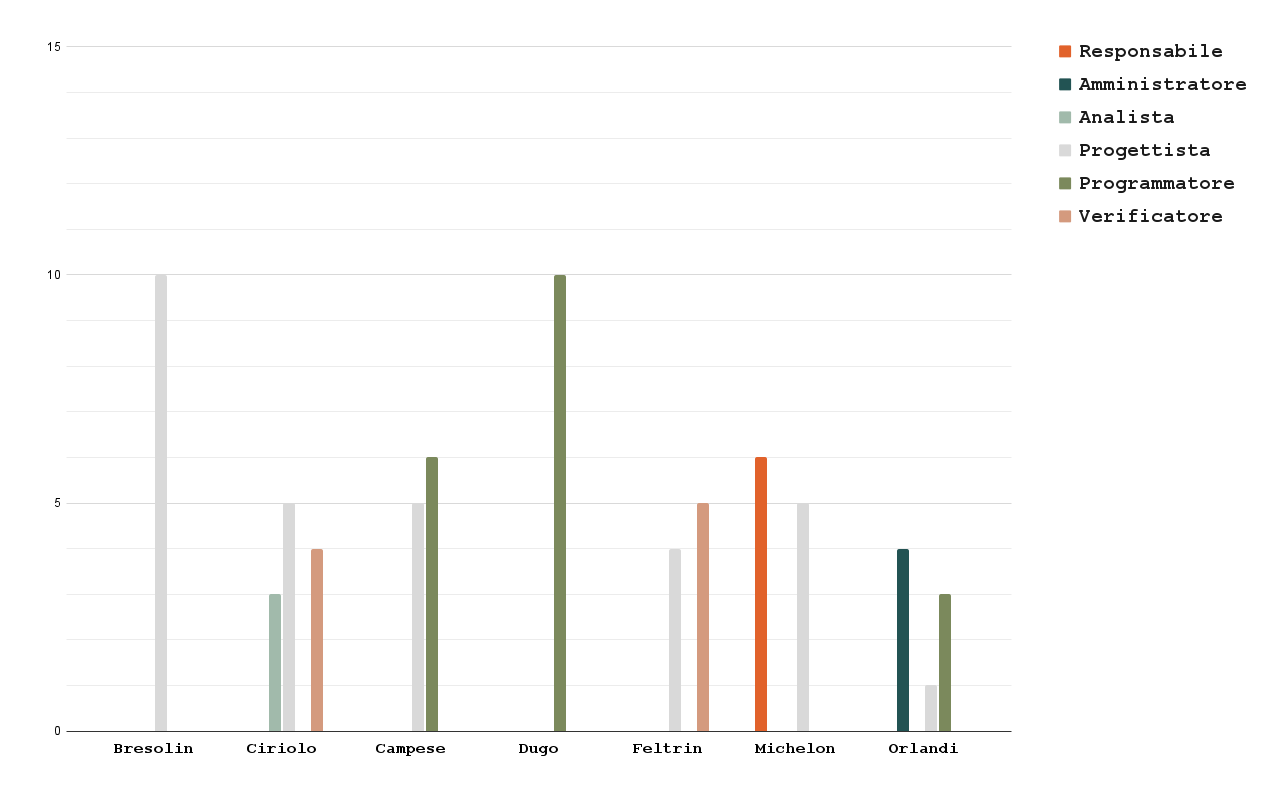
\includegraphics[width=15.5cm]{istogrammi/istogramma_5_periodo.png}
        \caption{Sprint 5 - Istogramma della ripartizione oraria dei ruoli. }
    \end{figure}

In questo incremento, il costo per ogni ruolo sarà come da tabella:
{\renewcommand{\arraystretch}{1.5}
\begin{table}[H]
\centering
\begin{tabularx}{0.42\textwidth}{c|c|c}

\textbf{Ruolo} & \textbf{Ore} & \textbf{Costo}\\
\hline
\textbf{Responsabile} & 6 & 180,00\texteuro\\
\hline
\textbf{Amministratore} & 4 & 80,00\texteuro \\
\hline
\textbf{Analista} & 3 & 75,00\texteuro \\
\hline
\textbf{Progettista} & 30 & 750,00\texteuro\\
\hline
\textbf{Programmatore} & 19 & 285,00 \texteuro \\ 
\hline
\textbf{Verificatore} & 9 & 135,00\texteuro \\ 
\hline
\rowcolor{primarycolor}
\textbf{Totale} & 71 & 1505,00\texteuro \\
\end{tabularx}
%}
\caption{Preventivo costi - Sprint 5}
\end{table}


La tabella è riassunta dal seguente aereogramma:
 \begin{figure}[H]
        \centering        
        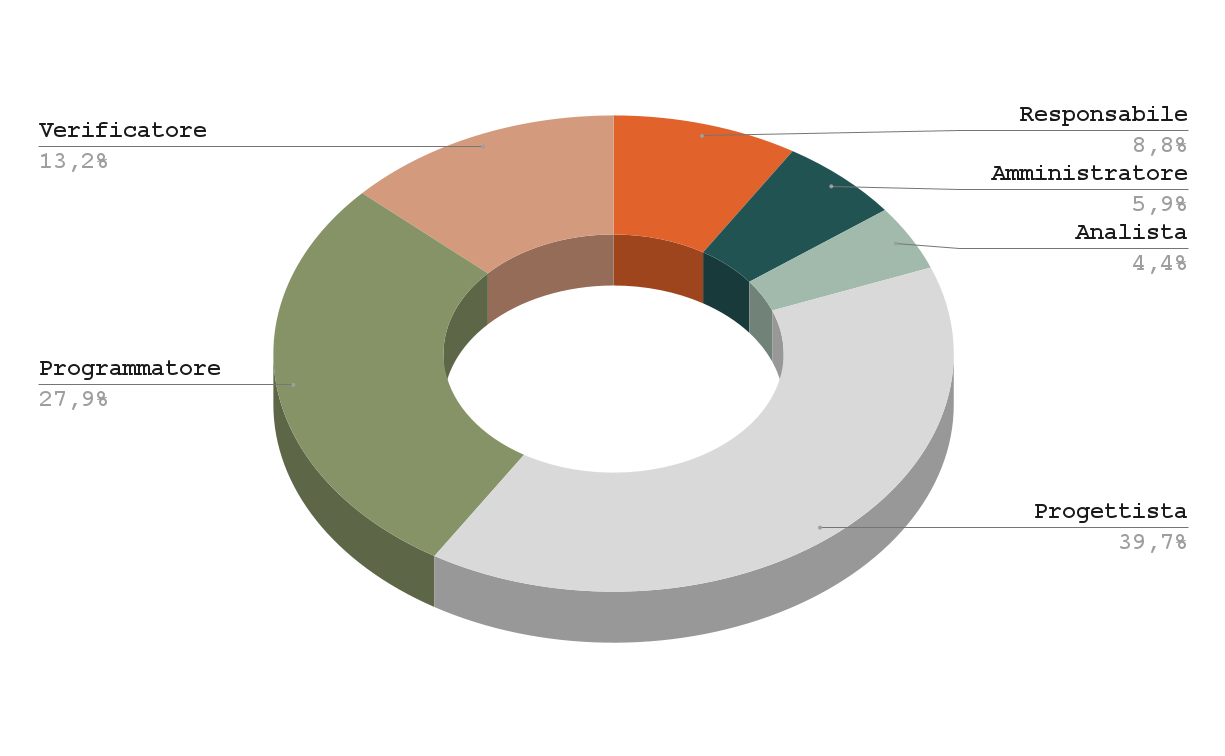
\includegraphics[width=15.5cm]{aereogrammi/areogramma_5_periodo.png}
        \caption{Sprint 5 - Areogramma della ripartizione oraria dei ruoli. }
    \end{figure}




%   PERIODO 6

\subsubsection{Sprint 6: da 2023-01-16 a 2024-01-30}
Di seguito, la distribuzione delle ore del sesto sprint; ogni componente del gruppo rivestirà i ruoli come segue:
\begin{table}[H]
\begin{tabularx}{\textwidth}{c|X|X|X|X|X|X|X}
        \textbf{Membri} & $\operatorname{\textbf{Re}}$ & $\mathrm{\textbf{Am}}$ & \textbf{An} & \textbf{Proj} & \textbf{Prgm} & \textbf{Ver} & \textbf{Totale} \\
        \hline Bresolin G. & 0 & 0 & 0 & 0 & \cellcolor{primarycolor}10 & 0 & 10 \\
        \hline Ciriolo I.  & 0 & 0 & 0 & 0 & \cellcolor{primarycolor}10 & 0 & 10 \\
        \hline Campese M.  & 0 & 0 & 0 & \cellcolor{primarycolor}6 & 0 & 0 & 6 \\
        \hline Dugo A.     & 0 & \cellcolor{primarycolor}4 & 1 & 0 & 0 & 3 & 8 \\
        \hline Feltrin E.  & 0 & 0 & 2 & \cellcolor{primarycolor}4 & 0 & 0 & 6 \\
        \hline Michelon R. & 0 & 0 & 0 & 2 & 0 & \cellcolor{primarycolor}7 & 9 \\
        \hline Orlandi G.  & \cellcolor{primarycolor}6 & 0 & 0 & 1 & 0 & 0 & 9 \\
        \hline
        \textbf{Totale ruolo} & 6 & 4 & 3 & 13 & 20 & 12 & 58 
    \end{tabularx}
    \caption{Preventivo ore - Sprint 6}
    \end{table}

La tabella è riassunta dal seguente istogramma:
 \begin{figure}[H]
        \centering        
        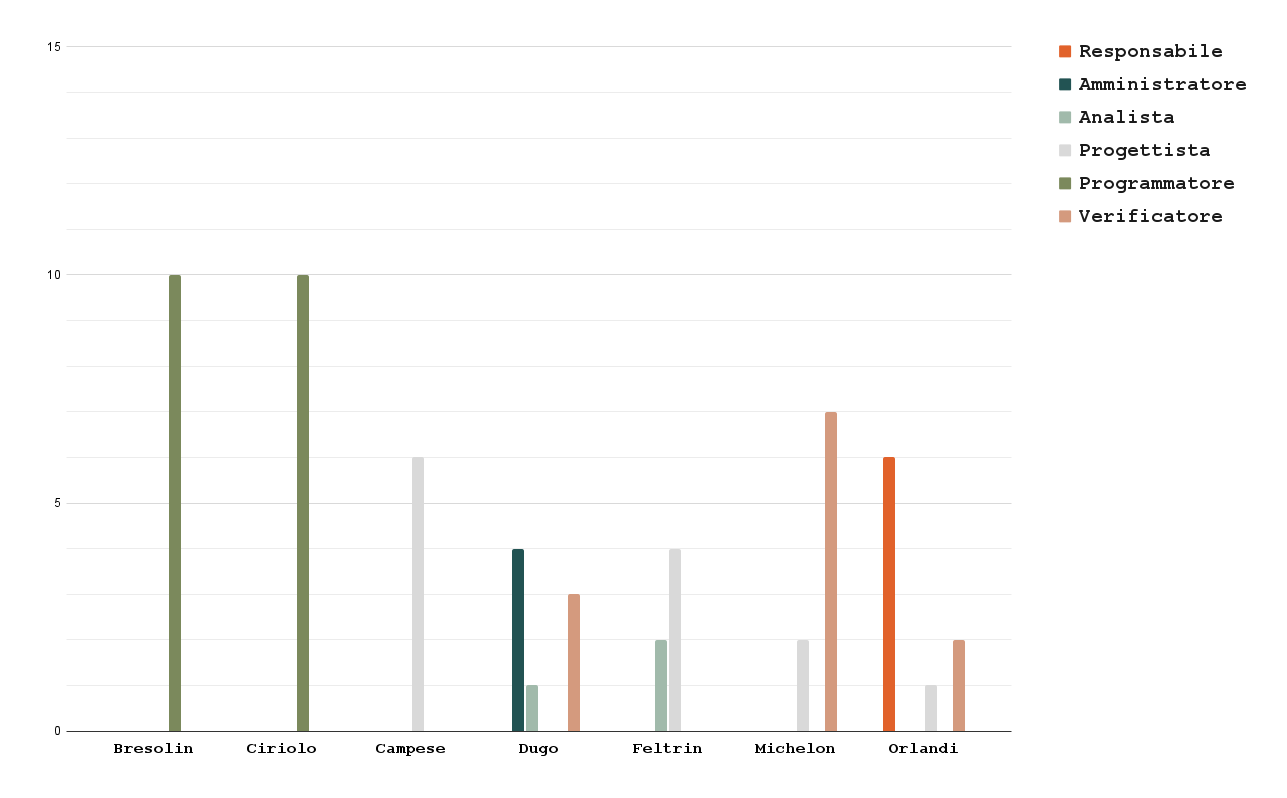
\includegraphics[width=15.5cm]{istogrammi/istogramma_6_periodo.png}
        \caption{Sprint 6 - Istogramma della ripartizione oraria dei ruoli. }
    \end{figure}


In questo incremento, il costo per ogni ruolo sarà come da tabella:
{\renewcommand{\arraystretch}{1.5}
\begin{table}[H]
\centering
\begin{tabularx}{0.42\textwidth}{c|c|c}

\textbf{Ruolo} & \textbf{Ore} & \textbf{Costo}\\
\hline
\textbf{Responsabile} & 6 & 180,00\texteuro\\
\hline
\textbf{Amministratore} & 4 & 80,00\texteuro \\
\hline
\textbf{Analista} & 3 & 75,00\texteuro \\
\hline
\textbf{Progettista} & 13 & 325,00\texteuro\\
\hline
\textbf{Programmatore} & 20 & 300,00 \texteuro \\ 
\hline
\textbf{Verificatore} & 12 & 180,00\texteuro \\ 
\hline
\rowcolor{primarycolor}
\textbf{Totale} & 58 & 1140,00\texteuro \\
\end{tabularx}
%}
\caption{Preventivo costi - Sprint 6}
\end{table}

La tabella è riassunta dal seguente aereogramma:
 \begin{figure}[H]
        \centering        
        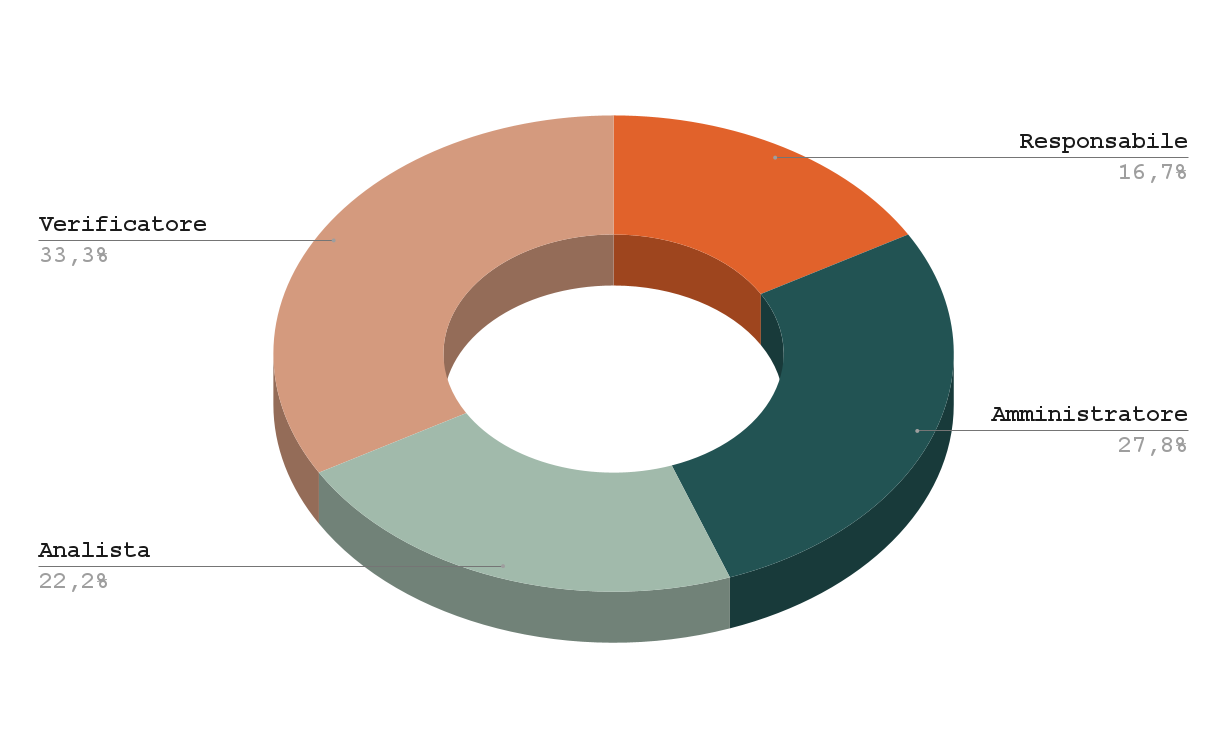
\includegraphics[width=15.5cm]{aereogrammi/areogramma_6_periodo.png}
        \caption{Sprint 6 - Areogramma della ripartizione oraria dei ruoli. }
    \end{figure}





%   PERIODO 7
\subsubsection{Sprint 7: da 2024-01-30 a 2024-02-13}
Di seguito, la distribuzione delle ore del settimo sprint; ogni componente del gruppo rivestirà i ruoli come segue:
\begin{table}[H]
\begin{tabularx}{\textwidth}{c|X|X|X|X|X|X|X}
        \textbf{Membri} & $\operatorname{\textbf{Re}}$ & $\mathrm{\textbf{Am}}$ & \textbf{An} & \textbf{Proj} & \textbf{Prgm} & \textbf{Ver} & \textbf{Tot} \\
        \hline Bresolin G. & \cellcolor{primarycolor}6 & 0 & 0 & 2 & 0 & 3 & 11 \\
        \hline Ciriolo I.  & 0 & \cellcolor{primarycolor}3 & 0 & 3 & 2 & 0 & 8 \\
        \hline Campese M.  & 0 & 0 & 0 & 1 & \cellcolor{primarycolor}11 & 0 & 12 \\
        \hline Dugo A.     & 0 & 0 & 1 & 3 & 0 & \cellcolor{primarycolor}5 & 9 \\
        \hline Feltrin E.  & 0 & 1 & 0 & \cellcolor{primarycolor}4 & 2 & 0 & 7 \\
        \hline Michelon R. & 0 & 0 & 1 & 0 & 0 & \cellcolor{primarycolor}4 & 5 \\
        \hline Orlandi G.  & 6 & 0 & 0 & 2 & \cellcolor{primarycolor}9 & 0 & 11 \\
        \hline
        \textbf{Totale ruolo} & 6 & 4 & 2 & 15 & 24 & 12 & 63 
    \end{tabularx}
    \caption{Preventivo ore - Sprint 7}
    \end{table}

La tabella è riassunta dal seguente istogramma:
 \begin{figure}[H]
        \centering        
        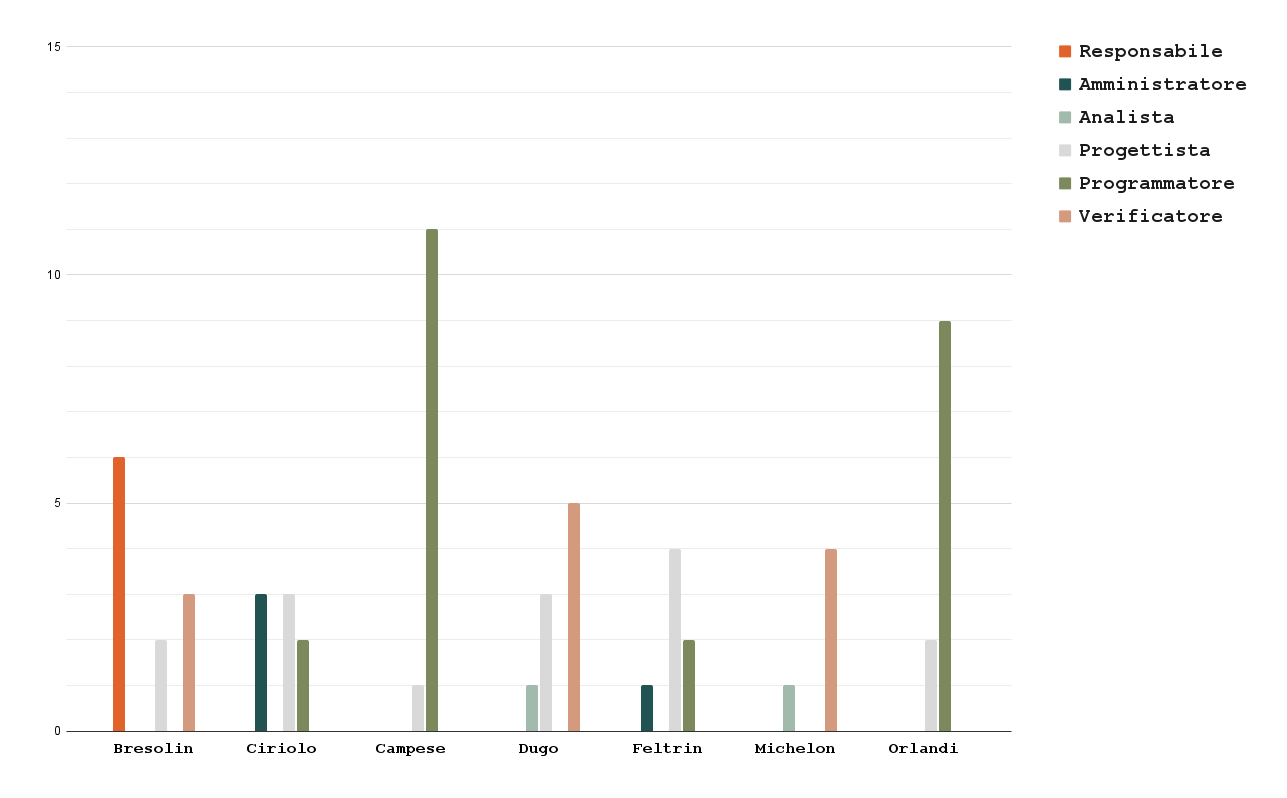
\includegraphics[width=15.5cm]{istogrammi/istogramma_7_periodo.png}
        \caption{Sprint 7- Istogramma della ripartizione oraria dei ruoli. }
    \end{figure}

In questo incremento, il costo per ogni ruolo sarà come da tabella:
{\renewcommand{\arraystretch}{1.5}
\begin{table}[H]
\centering
\begin{tabularx}{0.42\textwidth}{c|c|c}

\textbf{Ruolo} & \textbf{Ore} & \textbf{Costo}\\
\hline
\textbf{Responsabile} & 6 & 180,00\texteuro\\
\hline
\textbf{Amministratore} & 4 & 80,00\texteuro \\
\hline
\textbf{Analista} & 2 & 50,00\texteuro \\
\hline
\textbf{Progettista} & 15 & 375,00\texteuro\\
\hline
\textbf{Programmatore} & 24 & 360,00 \texteuro \\ 
\hline
\textbf{Verificatore} & 12 & 180,00\texteuro \\ 
\hline
\rowcolor{primarycolor}
\textbf{Totale} & 63 & 1225,00\texteuro \\
\end{tabularx}
%}
\caption{Preventivo costi - Sprint 7}
\end{table}

La tabella è riassunta dal seguente aereogramma:
 \begin{figure}[H]
        \centering        
        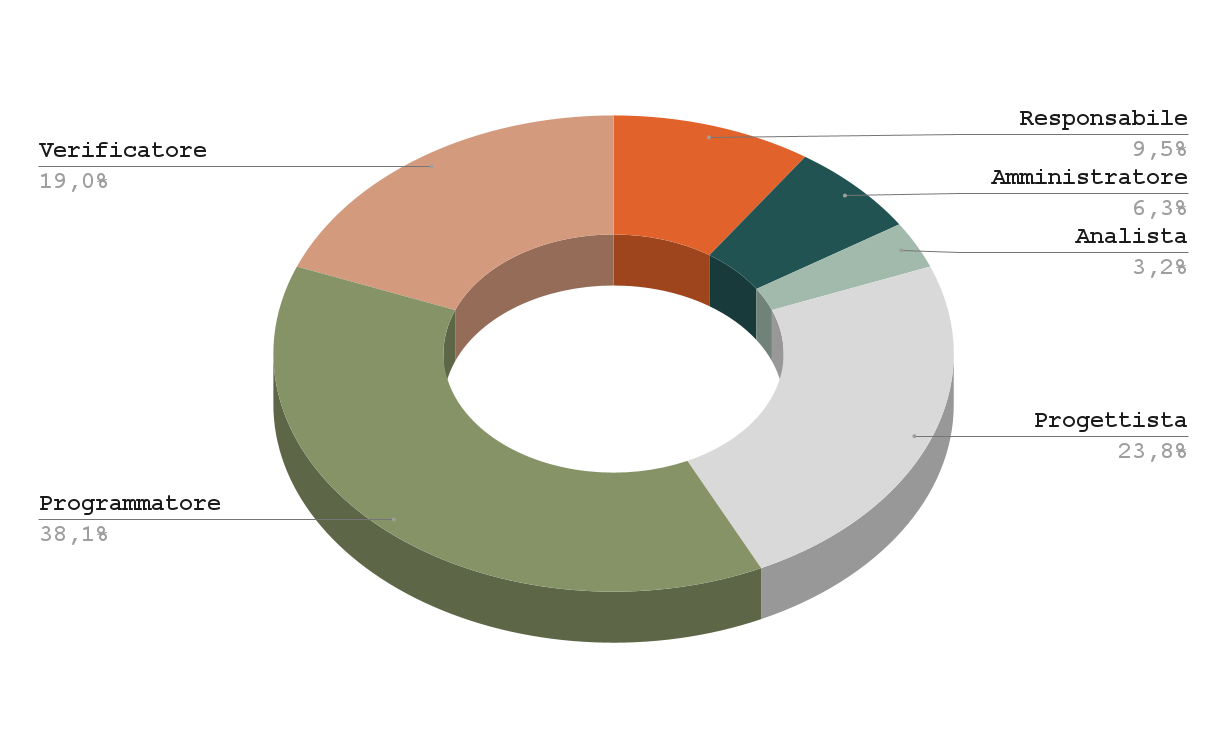
\includegraphics[width=15.5cm]{aereogrammi/areogramma_7_periodo.png}
        \caption{Sprint 7 - Areogramma della ripartizione oraria dei ruoli. }
    \end{figure}





%   PERIDO 8
\subsubsection{Sprint 8: da 2024-02-13 a 2024-02-27}
Di seguito, la distribuzione delle ore dell'ottavo sprint; ogni componente del gruppo rivestirà i ruoli come segue:
\begin{table}[H]
\begin{tabularx}{\textwidth}{c|X|X|X|X|X|X|X}
        \textbf{Membri} & $\operatorname{\textbf{Re}}$ & $\mathrm{\textbf{Am}}$ & \textbf{An} & \textbf{Proj} & \textbf{Prgm} & \textbf{Ver} & \textbf{Tot} \\
        \hline Bresolin G. & 0 & \cellcolor{primarycolor}4 & 0 & 0 & 3 & 0 & 7 \\
        \hline Ciriolo I.  & 4 & 0 & 0 & 0 & 0 & \cellcolor{primarycolor}5 & 9 \\
        \hline Campese M.  & 0 & 0 & 0 & 0 & 3 & \cellcolor{primarycolor}6 & 9 \\
        \hline Dugo A.     & \cellcolor{primarycolor}3 & 0 & 1 & 0 & 0 & 3 & 7 \\
        \hline Feltrin E.  & 0 & 0 & 0 & 0 & \cellcolor{primarycolor}10 & 0 & 10 \\
        \hline Michelon R. & 0 & 0 & 0 & 0 & \cellcolor{primarycolor}4 & 4 & 8 \\
        \hline Orlandi G.  & 0 & 0 & 0 & \cellcolor{primarycolor}8 & 4 & 0 & 12 \\
        \hline
        \textbf{Totale ruolo} & 7 & 4 & 1 & 8 & 24 & 18 & 62 
    \end{tabularx}
    \caption{Preventivo ore - Sprint 8}
    \end{table}

La tabella è riassunta dal seguente istogramma:
 \begin{figure}[H]
        \centering        
        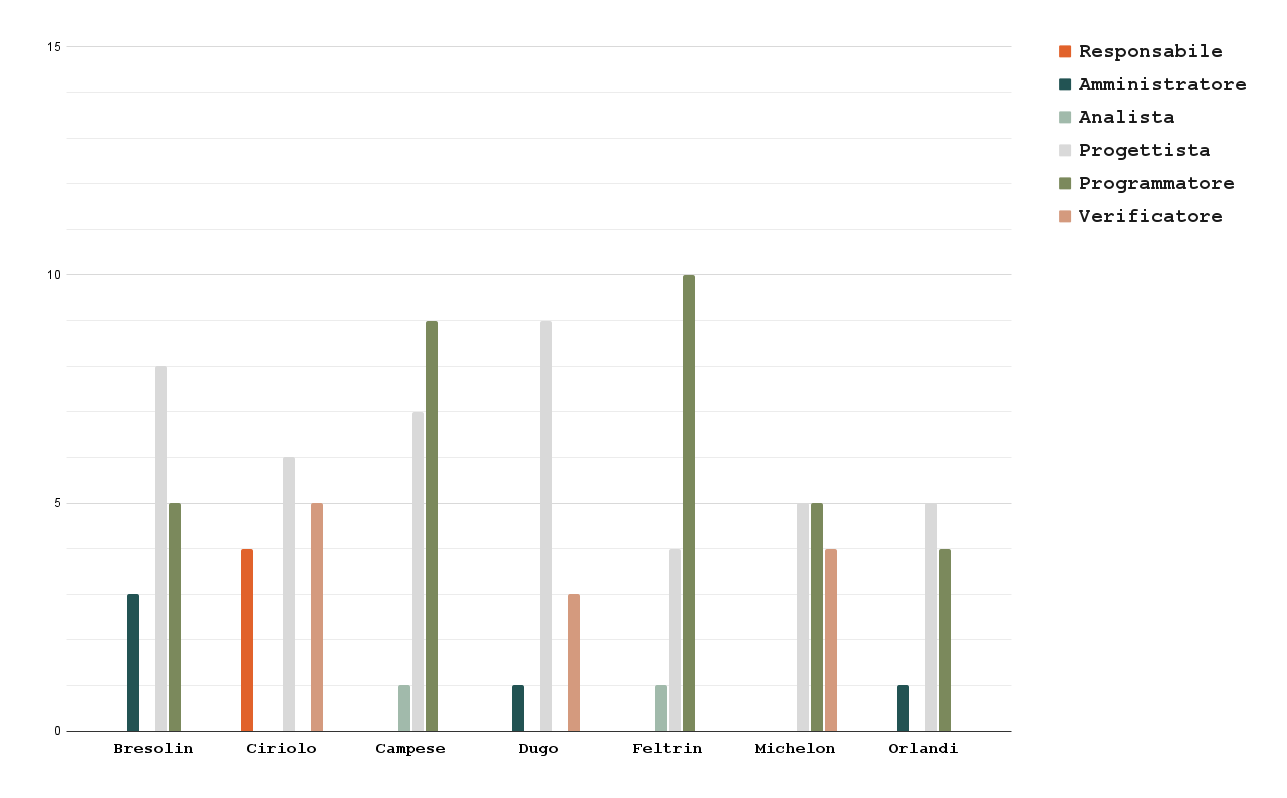
\includegraphics[width=15.5cm]{istogrammi/istogramma_8_periodo.png}
        \caption{Sprint 8 - Istogramma della ripartizione oraria dei ruoli. }
    \end{figure}


In questo incremento, il costo per ogni ruolo sarà come da tabella:
{\renewcommand{\arraystretch}{1.5}
\begin{table}[H]
\centering
\begin{tabularx}{0.42\textwidth}{c|c|c}

\textbf{Ruolo} & \textbf{Ore} & \textbf{Costo}\\
\hline
\textbf{Responsabile} & 7 & 180,00\texteuro\\
\hline
\textbf{Amministratore} & 4 & 80,00\texteuro \\
\hline
\textbf{Analista} & 1 & 25,00\texteuro \\
\hline
\textbf{Progettista} & 8 & 200,00\texteuro\\
\hline
\textbf{Programmatore} & 24 & 360,00 \texteuro \\ 
\hline
\textbf{Verificatore} & 18 & 270,00\texteuro \\ 
\hline
\rowcolor{primarycolor}
\textbf{Totale} & 62 & 1145,00\texteuro \\
\end{tabularx}
%}
\caption{Preventivo costi - Periodo 8}
\end{table}

La tabella è riassunta dal seguente aereogramma:
 \begin{figure}[H]
        \centering        
        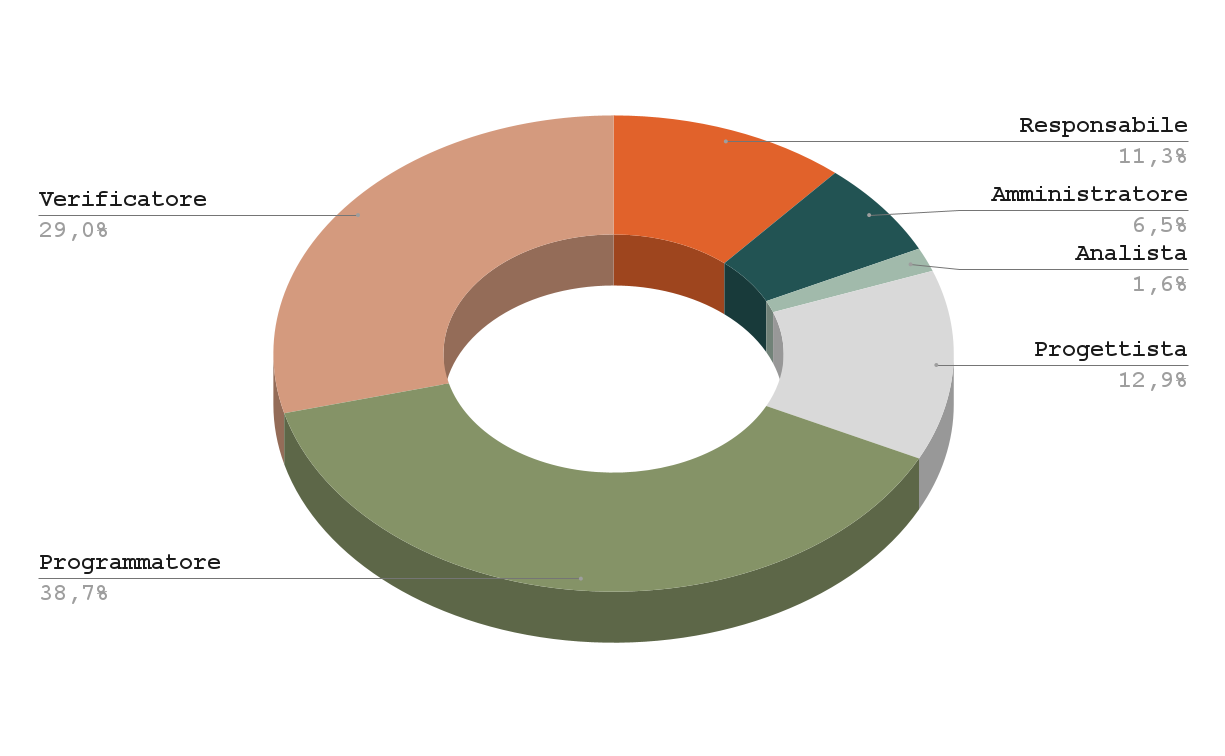
\includegraphics[width=15.5cm]{aereogrammi/areogramma_8_periodo.png}
        \caption{Sprint 8 - Areogramma della ripartizione oraria dei ruoli. }
    \end{figure}





%   PERIODO 9
\subsubsection{Sprint 9: da 2024-02-27 a 2024-03-12}
Di seguito, la distribuzione delle ore del nono sprint; ogni componente del gruppo rivestirà i ruoli come segue:
\begin{table}[H]
\begin{tabularx}{\textwidth}{c|X|X|X|X|X|X|X}
        \textbf{Membri} & $\operatorname{\textbf{Re}}$ & $\mathrm{\textbf{Am}}$ & \textbf{An} & \textbf{Proj} & \textbf{Prgm} & \textbf{Ver} & \textbf{Tot} \\
        \hline Bresolin G. & 0 & 0 & 0 & 0 & 0 & 10 & \cellcolor{primarycolor}10 \\
        \hline Ciriolo I.  & 0 & 0 & 0 & 0 & \cellcolor{primarycolor}12 & 0 & 12 \\
        \hline Campese M.  & 3 & \cellcolor{primarycolor}4 & 0 & 0 & 0 & 3 & 10 \\
        \hline Dugo A.     & 0 & 0 & 0 & 0 & 0 & \cellcolor{primarycolor}9 & 9 \\
        \hline Feltrin E.  & 0 & 0 & 0 & 0 & 2 & \cellcolor{primarycolor}4 & 6 \\
        \hline Michelon R. & 0 & 0 & 0 & 0 & \cellcolor{primarycolor}12 & 0 & 12 \\
        \hline Orlandi G.  & \cellcolor{primarycolor}3 & 0 & 0 & 2 & 3 & 1 & 9 \\
        \hline
        \textbf{Totale ruolo} & 6 & 4 & 0 & 2 & 29 & 27 & 68 
    \end{tabularx}
    \caption{Preventivo ore - Sprint 9}
    \end{table}

La tabella è riassunta dal seguente istogramma:
 \begin{figure}[H]
        \centering        
        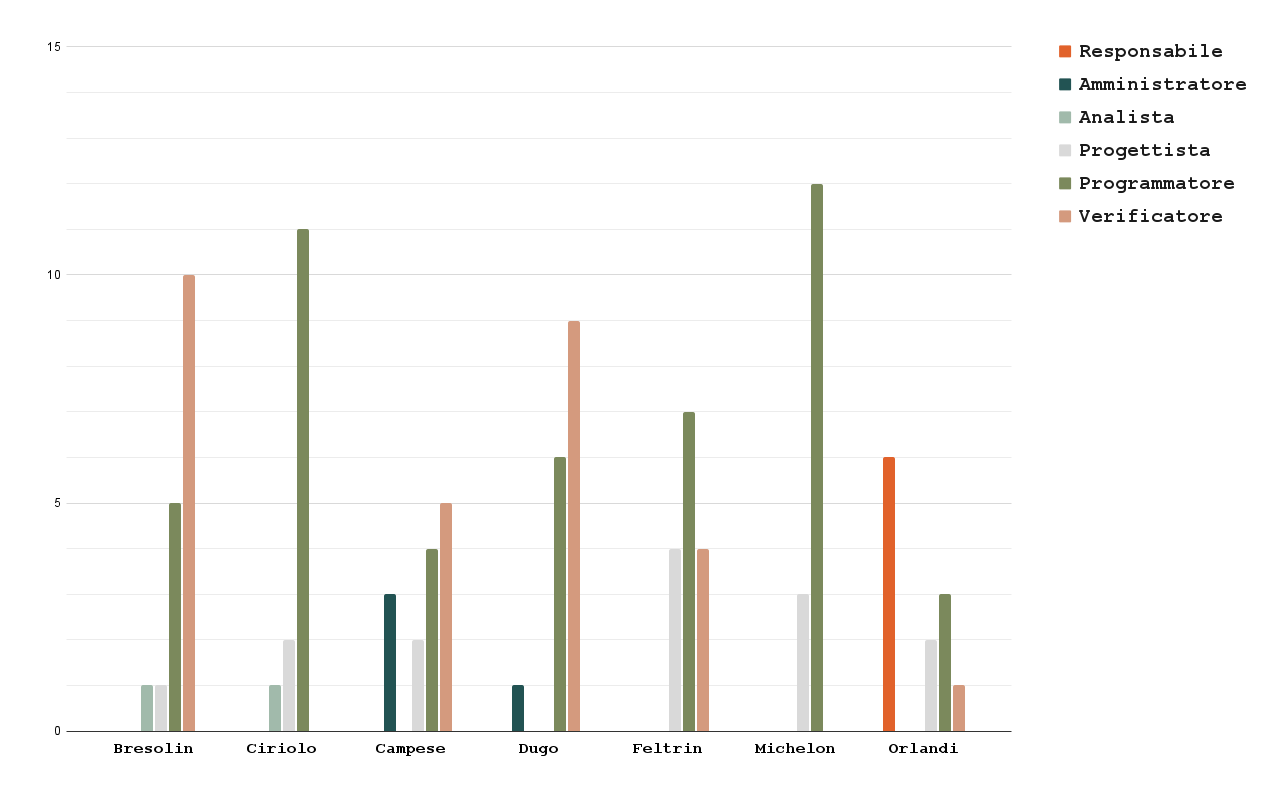
\includegraphics[width=15.5cm]{istogrammi/istogramma_9_periodo.png}
        \caption{Sprint 9 - Istogramma della ripartizione oraria dei ruoli. }
    \end{figure}

In questo incremento, il costo per ogni ruolo sarà come da tabella:
{\renewcommand{\arraystretch}{1.5}
\begin{table}[H]
\centering
\begin{tabularx}{0.42\textwidth}{c|c|c}

\textbf{Ruolo} & \textbf{Ore} & \textbf{Costo}\\
\hline
\textbf{Responsabile} & 6 & 180,00\texteuro\\
\hline
\textbf{Amministratore} & 4 & 80,00\texteuro \\
\hline
\textbf{Analista} & 0 & 0,00\texteuro \\
\hline
\textbf{Progettista} & 2 & 50,00\texteuro\\
\hline
\textbf{Programmatore} & 29 & 435,00\texteuro \\ 
\hline
\textbf{Verificatore} & 27 & 405,00\texteuro \\ 
\hline
\rowcolor{primarycolor}
\textbf{Totale} & 68 & 1150,00\texteuro \\
\end{tabularx}
%}
\caption{Preventivo costi - Sprint 9}
\end{table}

La tabella è riassunta dal seguente aereogramma:
 \begin{figure}[H]
        \centering        
        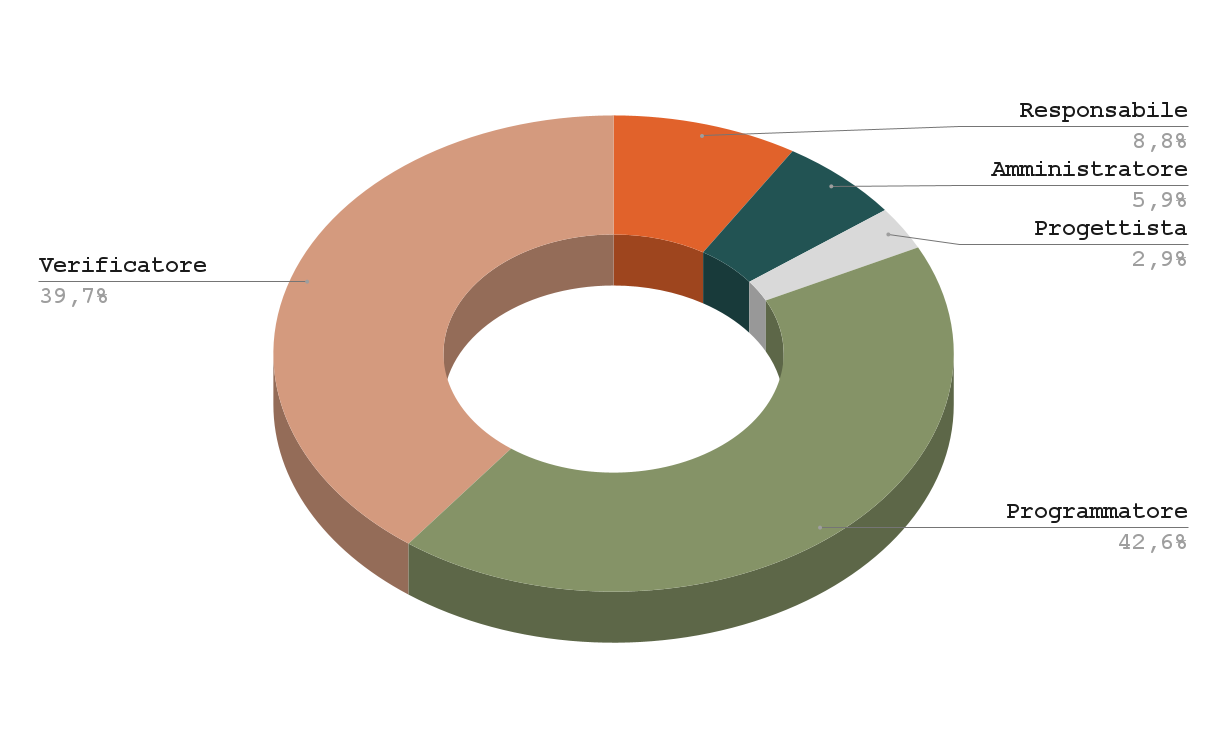
\includegraphics[width=15.5cm]{aereogrammi/areogramma_9_periodo.png}
        \caption{Sprint 9 - Areogramma della ripartizione oraria dei ruoli. }
    \end{figure}




%   PERIODO 10

\subsubsection{Sprint 10: da 2024-03-12 a 2024-03-26}
Di seguito, la distribuzione delle ore del decimo sprint; ogni componente del gruppo rivestirà i ruoli come segue:
\begin{table}[H]
\begin{tabularx}{\textwidth}{c|X|X|X|X|X|X|X}
        \textbf{Membri} & $\operatorname{\textbf{Re}}$ & $\mathrm{\textbf{Am}}$ & \textbf{An} & \textbf{Proj} & \textbf{Prgm} & \textbf{Ver} & \textbf{Tot} \\
        \hline Bresolin G. & 3 & 0 & 0 & 0 & \cellcolor{primarycolor}10 & 0 & 13 \\
        \hline Ciriolo I.  & 0 & 0 & 0 & 0 & 2 & \cellcolor{primarycolor}3 & 5 \\
        \hline Campese M.  & 0 & 0 & 0 & 0 & \cellcolor{primarycolor}5 & 0 & 5 \\
        \hline Dugo A.     & 0 & 0 & 0 & 0 & \cellcolor{primarycolor}7 & 4 & 11 \\
        \hline Feltrin E.  & 0 & 2 & 0 & 0 & 0 & \cellcolor{primarycolor}9 & 11 \\
        \hline Michelon R. & \cellcolor{primarycolor}3 & 2 & 0 & 0 & 1 & 4 & 10 \\
        \hline Orlandi G.  & 0 & 0 & 0 & 0 & 0 & \cellcolor{primarycolor}7 & 7 \\
        \hline
        \textbf{Totale ruolo} & 6 & 4 & 0 & 0 & 25 & 27 & 62 
    \end{tabularx}
    \caption{Preventivo ore - Sprint 10}
    \end{table}

La tabella è riassunta dal seguente istogramma:
 \begin{figure}[H]
        \centering        
        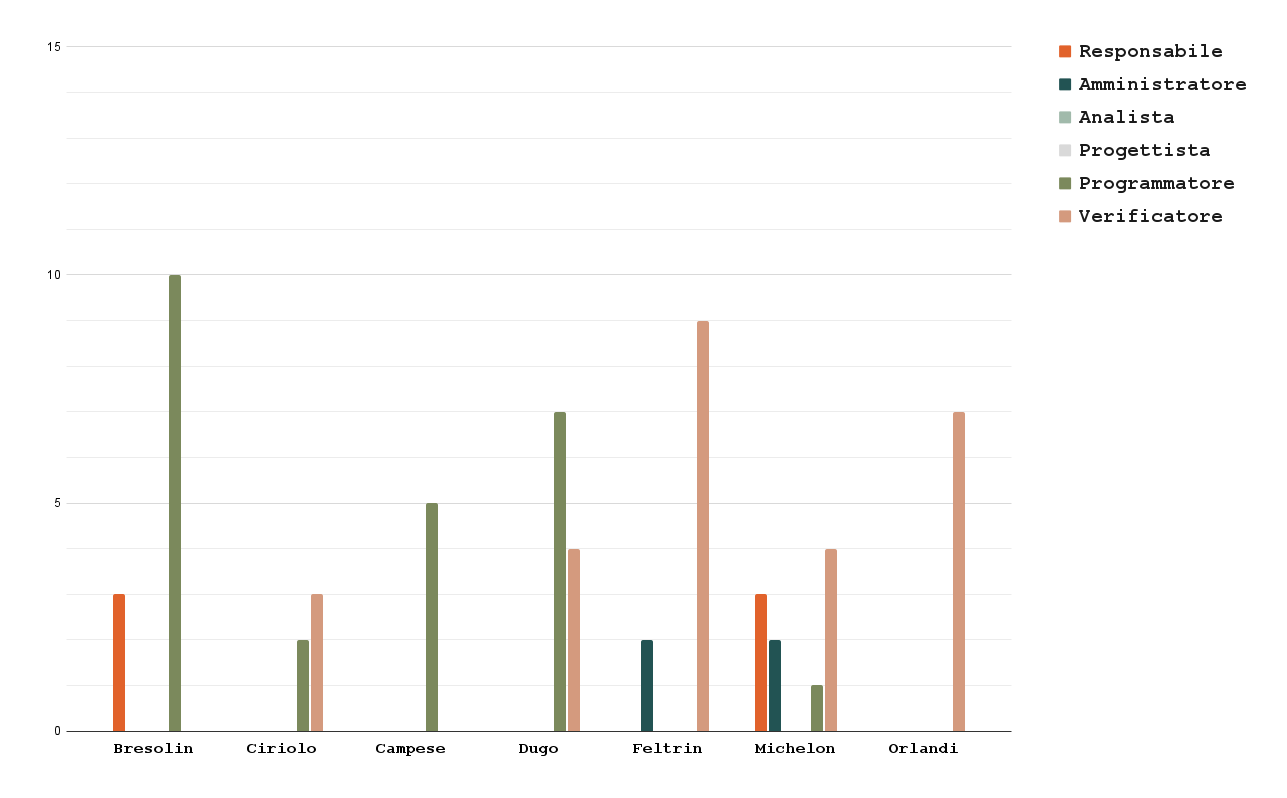
\includegraphics[width=15.5cm]{istogrammi/istogramma_10_periodo.png}
        \caption{Sprint 10 - Istogramma della ripartizione oraria dei ruoli. }
    \end{figure}

In questo incremento, il costo per ogni ruolo sarà come da tabella:
{\renewcommand{\arraystretch}{1.5}
\begin{table}[H]
\centering
\begin{tabularx}{0.42\textwidth}{c|c|c}

\textbf{Ruolo} & \textbf{Ore} & \textbf{Costo}\\
\hline
\textbf{Responsabile} & 6 & 180,00\texteuro\\
\hline
\textbf{Amministratore} & 4 & 80,00\texteuro \\
\hline
\textbf{Analista} & 0 & 0,00\texteuro \\
\hline
\textbf{Progettista} & 0 & 0,00\texteuro\\
\hline
\textbf{Programmatore} & 25 & 375,00\texteuro \\ 
\hline
\textbf{Verificatore} & 27 & 405,00\texteuro \\ 
\hline
\rowcolor{primarycolor}
\textbf{Totale} & 62 & 1040,00\texteuro \\
\end{tabularx}
%}
\caption{Preventivo costi - Sprint 10}
\end{table}

La tabella è riassunta dal seguente aereogramma:
 \begin{figure}[H]
        \centering        
        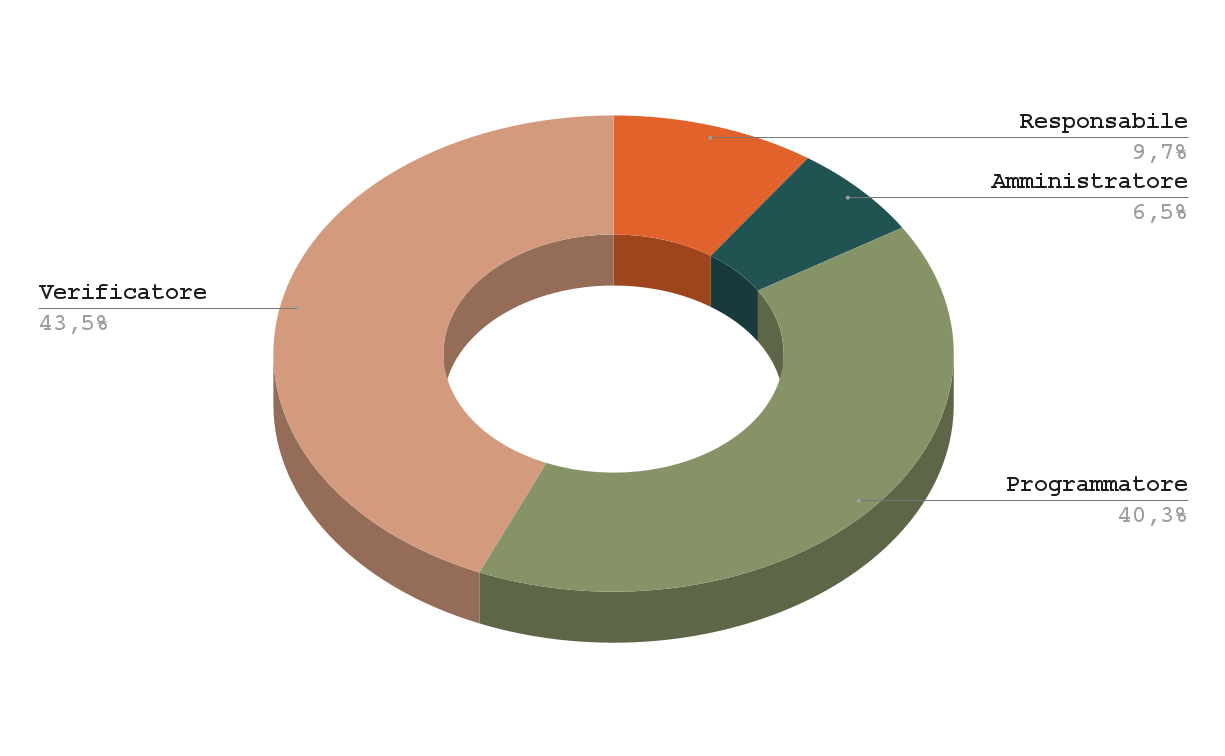
\includegraphics[width=15.5cm]{aereogrammi/areogramma_10_periodo.png}
        \caption{Sprint 10 - Areogramma della ripartizione oraria dei ruoli. }
    \end{figure}



%   PERIODO 11
\subsubsection{Sprint 11: da 2024-03-26 a 2024-04-08}
Di seguito, la distribuzione delle ore dell'undicesimo sprint; ogni componente del gruppo rivestirà i ruoli come segue:
\begin{table}[H]
\begin{tabularx}{\textwidth}{c|X|X|X|X|X|X|X}
        \textbf{Membri} & $\operatorname{\textbf{Re}}$ & $\mathrm{\textbf{Am}}$ & \textbf{An} & \textbf{Proj} & \textbf{Prgm} & \textbf{Ver} & \textbf{Tot} \\
        \hline Bresolin G. & 0 & 0 & 0 & 0 & 1 & \cellcolor{primarycolor}4 & 5 \\
        \hline Ciriolo I.  & 0 & \cellcolor{primarycolor}4 & 0 & 0 & 1 & 2 & 7 \\
        \hline Campese M.  & 1 & 1 & 0 & 0 & 1 & \cellcolor{primarycolor}2,5 & 5,5 \\
        \hline Dugo A.     & \cellcolor{primarycolor}2 & 0 & 0 & 0 & 2 & 0 & 4 \\
        \hline Feltrin E.  & 3 & 1 & 0 & 0 & 0 & \cellcolor{primarycolor}5 & 9 \\
        \hline Michelon R. & 0 & 0 & 0 & 0 & 0 & \cellcolor{primarycolor}5 & 5 \\
        \hline Orlandi G.  & 0 & 3 & 0 & 0 & \cellcolor{primarycolor}3 & 3 & 9 \\
        \hline
        \textbf{Totale ruolo} & 6 & 9 & 0 & 0 & 8 & 21,5 & 44,5 
    \end{tabularx}
    \caption{Preventivo ore - Sprint 11}
\end{table}

La tabella è riassunta dal seguente istogramma:
\begin{figure}[H]
        \centering        
        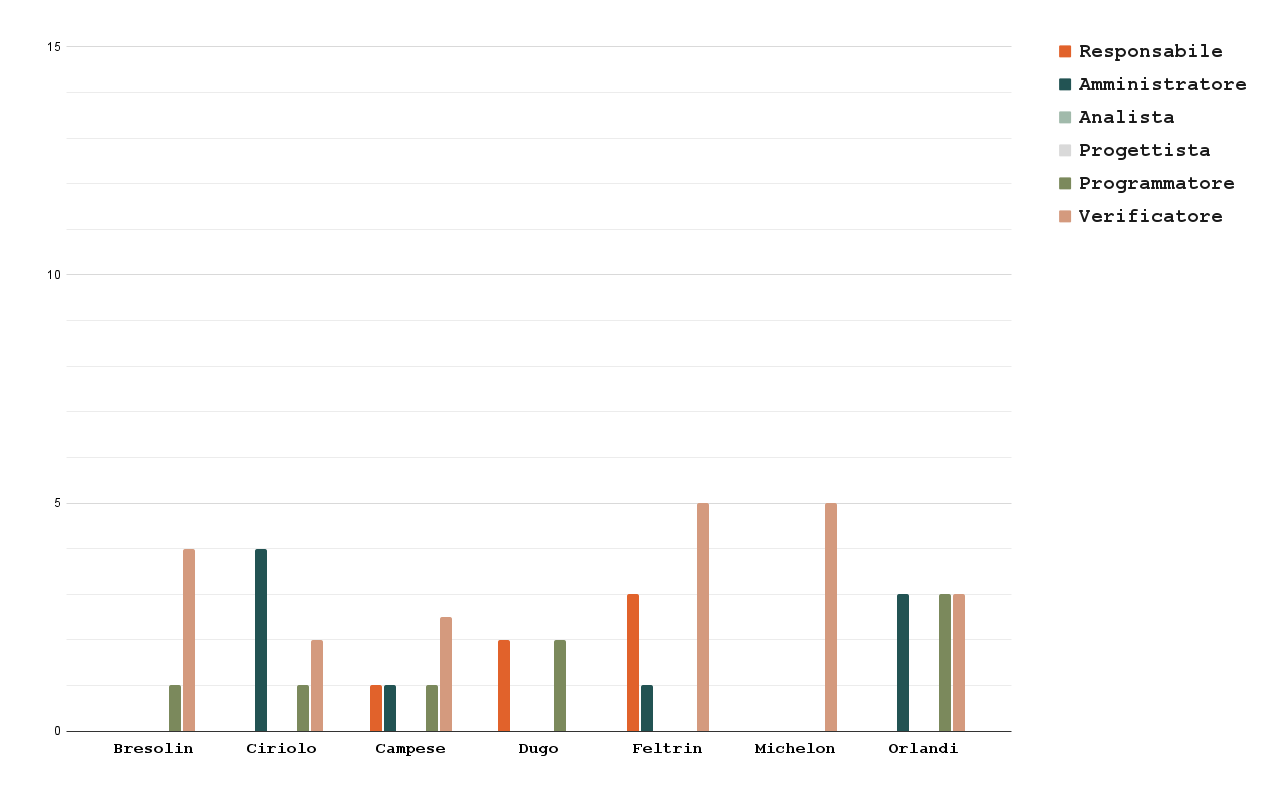
\includegraphics[width=15.5cm]{istogrammi/istogramma_11_periodo.png}
        \caption{Sprint 11 - Istogramma della ripartizione oraria dei ruoli. }
\end{figure}

In questo incremento, il costo per ogni ruolo sarà come da tabella:
{\renewcommand{\arraystretch}{1.5}
\begin{table}[H]
\centering
\begin{tabularx}{0.42\textwidth}{c|c|c}

\textbf{Ruolo} & \textbf{Ore} & \textbf{Costo}\\
\hline
\textbf{Responsabile} & 6 & 180,00\texteuro\\
\hline
\textbf{Amministratore} & 9 & 80,00\texteuro \\
\hline
\textbf{Analista} & 0 & 0,00\texteuro \\
\hline
\textbf{Progettista} & 0 & 0,00\texteuro\\
\hline
\textbf{Programmatore} & 8 & 120,00\texteuro \\ 
\hline
\textbf{Verificatore} & 21,5 & 322,50\texteuro \\ 
\hline
\rowcolor{primarycolor}
\textbf{Totale} & 44,5 & 802,50\texteuro \\
\end{tabularx}
%}
\caption{Preventivo costi - Sprint 11}
\end{table}
La tabella è riassunta dal seguente aereogramma:
 \begin{figure}[H]
        \centering        
        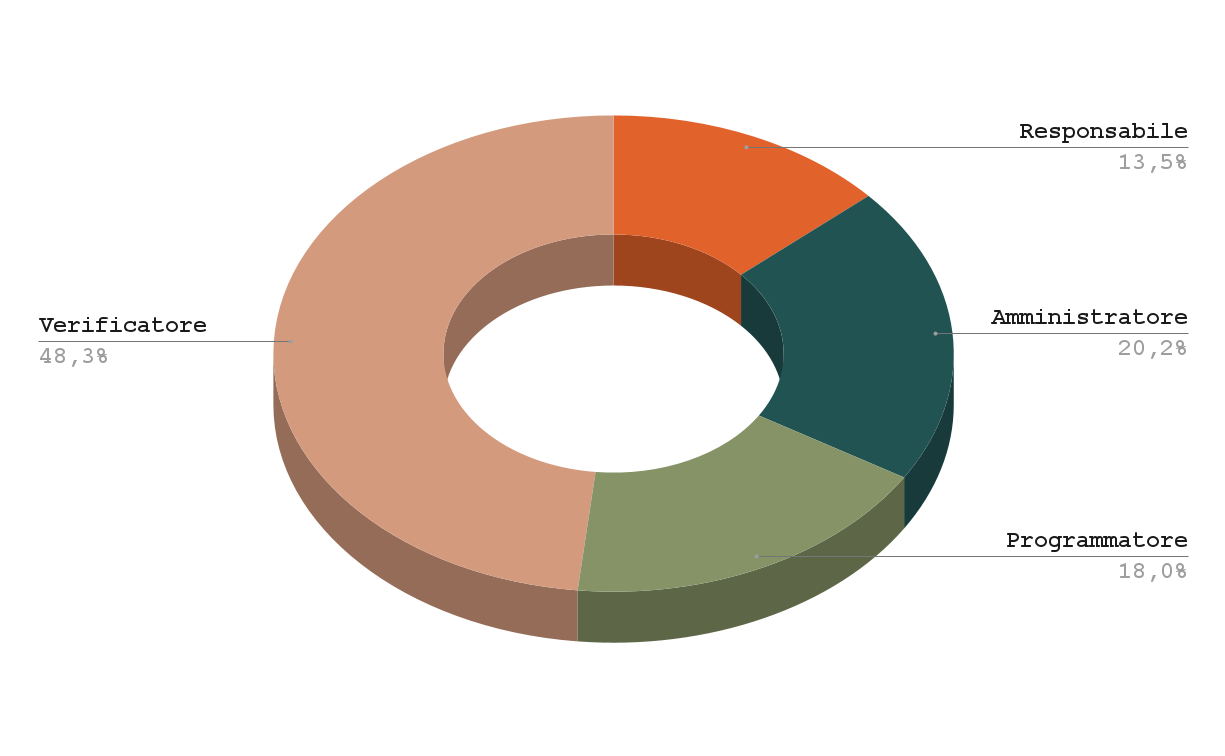
\includegraphics[width=15.5cm]{aereogrammi/areogramma_11_periodo.png}
        \caption{Sprint 11 - Areogramma della ripartizione oraria dei ruoli. }
    \end{figure}



\newpage
%   CONSUNTIVO

\section{Consuntivo}

% PERIODO 1 CONSUNTIVO
\subsubsection{Sprint 1: da 2023-11-07 a 2023-11-21}
Di seguito, la distribuzione delle ore del primo sprint; ogni componente del gruppo ha rivestito i ruoli come segue:
\begin{table}[H]
\begin{tabularx}{\textwidth}{c|X|X|X|X|X|X|X}
        \textbf{Membri} & $\operatorname{\textbf{Re}}$ & $\mathrm{\textbf{Am}}$ & \textbf{An} & \textbf{Proj} & \textbf{Prgm} & \textbf{Ver} & \textbf{Tot} \\
        \hline Bresolin G. & 0 & 5 & 0 & 0 & 0 & 0 & 5 \\
        \hline Ciriolo I.  & 0 & 0 & 7 & 0 & 0 & 1 & 8 \\
        \hline Campese M.  & 0 & 0 & 2 & 0 & 0 & 7 & 9 \\
        \hline Dugo A.     & 0 & 5 & 0 & 0 & 0 & 0 & 5 \\
        \hline Feltrin E.  & 7 & 1 & 0 & 0 & 0 & 0 & 8 \\
        \hline Michelon R. & 0 & 6 & 0 & 0 & 0 & 0 & 6 \\
        \hline Orlandi G.  & 0 & 0 & 3 & 0 & 0 & 1 & 4 \\
        \hline
        \textbf{Totale ruolo} & 2 & 17 & 12 & 0 & 0 & 9 & 45 
    \end{tabularx}
    \caption{Consuntivo ore - Sprint 1}
    \end{table}


\begin{table}[H]
\begin{tabularx}{\textwidth}{c|X|X|X|X|X|X|X}
        \textbf{Ruolo} & \textbf{Ore preventivo} & \textbf{Ore consuntivo} & \textbf{Delta ore} & \textbf{Costo preventivo} & \textbf{Costo consuntivo} & \textbf{Delta costo} \\
        \hline
        \textbf{RES} & 8 & 7 & 1 & 240,00\texteuro & € 210,00\texteuro & € 30,00\texteuro \\
        \hline
        \textbf{AMM} & 15 & 17 & -2 & 300,00\texteuro & 340,00\texteuro & -€ 40,00\texteuro \\
        \hline
        \textbf{AN} & 11 & 12 & -1 & 275,00\texteuro & 300,00\texteuro & -€ 25,00\texteuro \\
        \hline
        \textbf{PROJ} & 0 & 0 & 0 & 0,00\texteuro & 0,00\texteuro & € 0,00\texteuro \\
        \hline
        \textbf{PROG} & 0 & 0 & 0 & 0,00\texteuro & € 0,00 & € 0,00\texteuro \\
        \hline
        \textbf{VER} & 10 & 9 & 1 & 150,00\texteuro & € 135,00 & € 15,00\texteuro \\
        \hline
        \rowcolor{primarycolor}
        \textbf{TOT} & 44 & 45 & -1 & 965,00\texteuro & 985,00\texteuro & -20,00\texteuro
    \end{tabularx}
    \caption{Consuntivo costi - Sprint 2}
\end{table}
\subsubsubsection{Retrospettiva dell'incremento}
Il team nel primo sprint ha svolto le seguenti attività:
\begin{itemize}
    \item Stilato Piano di progetto;
    \item Automatizzato versionamento repository;
    \item Prima stesura Analisi dei requisiti;
    \item Stilato verbali relativi allo sprint.
\end{itemize}
\subsubsubsection{Considerazioni}
\begin{itemize}
\item Il consuntivo di periodo possiede delle discrepanze rispetto al preventivo stilato. Questo è dovuto alla sottostima delle tempistiche per alcune attività onerose che si sono rivelate più importanti dal punto di vista delle ore necessarie;
\item A seguito di incomprensioni tra le componenti del gruppo, sono state stilate in maniera non sufficiente alcune sezioni del Piano di Qualifica; questo ha comportato un ritardo e un aggiornamento della pianificazione che tenesse conto della nuova stesura del documento.
\end{itemize}
%PERIODO 2 CONSUNTIVO


\subsubsection{Sprint 2: da 2023-11-21 a 2023-12-05}
Di seguito, la distribuzione delle ore del secondo sprint; ogni componente del gruppo ha rivestito i ruoli come segue:
\begin{table}[H]
\begin{tabularx}{\textwidth}{c|X|X|X|X|X|X|X}
        \textbf{Membri} & $\operatorname{\textbf{Re}}$ & $\mathrm{\textbf{Am}}$ & \textbf{An} & \textbf{Proj} & \textbf{Prgm} & \textbf{Ver} & \textbf{Totale} \\
        \hline Bresolin G. & 0 & 1 & 7 & 0 & 0 & 0 & 8 \\
        \hline Ciriolo I.  & 7 & 0 & 0 & 0 & 0 & 1 & 8 \\
        \hline Campese M.  & 0 & 4 & 2 & 0 & 0 & 1,5 & 7,5 \\
        \hline Dugo A.     & 0 & 0 & 2 & 2 & 9 & 0 & 13 \\
        \hline Feltrin E.  & 0 & 0 & 0 & 0 & 11 & 0 & 11 \\
        \hline Michelon R. & 0 & 0 & 2 & 1 & 13 & 0 & 16 \\
        \hline Orlandi G.  & 0 & 0 & 0 & 0 & 0 & 7 & 7 \\
        \hline
        \textbf{Totale ruolo} & 7 & 5 & 13 & 3 & 33 & 9,5 & 70,5 
    \end{tabularx}
    \caption{Consuntivo ore - Sprint 2}
    \end{table}

 
\begin{table}[H]
\begin{tabularx}{\textwidth}{c|X|X|X|X|X|X|X}
        \textbf{Ruolo} & \textbf{Ore preventivo} & \textbf{Ore consuntivo} & \textbf{Delta orario} & \textbf{Costo preventivo} & \textbf{Costo consuntivo} & \textbf{Delta costo} \\
        \hline
        \textbf{RES} & 7 & 7 & 0 & 210,00\texteuro & 210,00\texteuro &  0,00\texteuro \\
        \hline
        \textbf{AMM} & 6 & 5 & 1 & 120,00\texteuro & 100,00\texteuro & 20,00\texteuro \\
        \hline
        \textbf{AN} & 12 & 13 & -1 & 300,00\texteuro & 325,00\texteuro & -25,00\texteuro \\
        \hline
        \textbf{PROJ} & 3 & 3 & 0 & 75,00\texteuro & 75,00\texteuro & 0,00\texteuro \\
        \hline
        \textbf{PROG} & 33 & 33 & 0 & 495,00\texteuro & 495,00\texteuro & 0,00\texteuro \\
        \hline
        \textbf{VER} & 9,5 & 9,5 & 0 & 142,50\texteuro & 142,50\texteuro & 0,00\texteuro \\
        \hline
        \rowcolor{primarycolor}
        \textbf{TOT} & 70,5 & 70,5 & 0 & 1342,50\texteuro & 1347,50\texteuro & -5,00\texteuro 
    \end{tabularx}
    \caption{Consuntivo ore e costi - Sprint 2}
\end{table}
\subsubsubsection{Retrospettiva dell'incremento}
Il team nel primo sprint ha svolto le seguenti attività:
\begin{itemize}
    \item Codifica dei vari PoC;
    \item Aggiornamento Norme di progetto;
    \item Aggiornamento Piano di progetto;
    \item Prima stesura Piano di qualifica;
    \item Stesura iniziale Analisi dei requisiti;
    \item Stilato verbali relativi allo sprint.
\end{itemize}
\subsubsubsection{Considerazioni}
\begin{itemize}
    \item Il consuntivo del secondo sprint risulta più conforme rispetto al primo, con solamente 5 euro spesi in più rispetto al preventivo. Si può quindi affermare che il preventivo ipotizzato per il secondo sprint è conforme e si rispecchia con il consuntivo;
    \item L'unico appunto che può essere fatto è legato alla sottostima delle ore del ruolo dell'analista.
\end{itemize}
\subsubsection{Sprint 3: da 2023-12-05 a 2023-12-19}
Di seguito, la distribuzione delle ore del terzo sprint; ogni componente del gruppo ha rivestito i ruoli come segue:

\begin{table}[H]
    \begin{tabularx}{\textwidth}{c|X|X|X|X|X|X|X}
        \textbf{Membri} & $\operatorname{\textbf{Re}}$ & $\mathrm{\textbf{Am}}$ & \textbf{An} & \textbf{Proj} & \textbf{Prgm} & \textbf{Ver} & \textbf{Totale} \\
        \hline Bresolin G. & 0 & 0 & 2 & 1 & 0 & 7 & 10 \\
        \hline Ciriolo I.  & 0 & 4 & 1 & 0 & 0 & 3 & 8 \\
        \hline Campese M.  & 0 & 0 & 2 & 0 & 0 & 4 & 6 \\
        \hline Dugo A.     & 6 & 1 & 3 & 0 & 0 & 0 & 10 \\
        \hline Feltrin E.  & 0 & 0 & 8 & 0 & 0 & 0 & 8 \\
        \hline Michelon R. & 0 & 0 & 6 & 0 & 0 & 0 & 6 \\
        \hline Orlandi G.  & 0 & 0 & 3 & 0 & 3 & 0 & 6 \\
        \hline
        \textbf{Totale ruolo} & 6 & 5 & 23 & 1 & 3 & 14 & 52 
    \end{tabularx}
    \caption{Consuntivo ore - Sprint 3}
\end{table}

\begin{table}[H]
    \begin{tabularx}{\textwidth}{c|X|X|X|X|X|X|X}
        \textbf{Ruolo} & \textbf{Ore preve} & \textbf{Ore consu} & \textbf{Delta ore} & \textbf{Costo preve} & \textbf{Costo consu} & \textbf{Delta costo} \\
        \hline
        \textbf{RES} & 6 & 6 & 0 & 180,00\texteuro & 180,00\texteuro & 0,00\texteuro \\
        \hline
        \textbf{AMM} & 4 & 5 & -1 & 80,00\texteuro & 100,00\texteuro & 20,00\texteuro \\
        \hline
        \textbf{AN} & 25 & 23 & 2 & 625,00\texteuro & 575,00\texteuro & 50,00\texteuro \\
        \hline
        \textbf{PROJ} & 1 & 1 & 0 & 25,00\texteuro & 25,00\texteuro & 0,00\texteuro \\
        \hline
        \textbf{PROG} & 4 & 3 & 1 & 60,00\texteuro & 45,00\texteuro & -15,00\texteuro \\
        \hline
        \textbf{VER} & 14 & 14 & 0 & 210,00\texteuro & 210,00\texteuro & 0,00\texteuro \\
        \hline
        \rowcolor{primarycolor}
        \textbf{TOT} & 54 & 52 & 2 & 1.180,00\texteuro & 1.135,00\texteuro & 45,00\texteuro \\
    \end{tabularx}
    \caption{Consuntivo ore e costi - Sprint 3}
\end{table}
\subsubsubsection{Retrospettiva dell'incremento}
Il team nel primo sprint ha svolto le seguenti attività:
\begin{itemize}
    \item Codifica del PoC finale;
    \item Aggiornamento Norme di progetto;
    \item Aggiornamento Piano di progetto;
    \item Aggiornamento Piano di qualifica;
    \item Ristrutturazione Analisi dei requisiti;
    \item Stilato verbali relativi allo sprint.
\end{itemize}
\subsubsubsection{Considerazioni}
\begin{itemize}
    \item Nel terzo sprint il team ha lavorato in maniera efficace ed efficiente, rispettando le scadenze e completando le task assegnate nei tempi previsti;
    \item Anche in questo caso come nel precedente vi è una sottostima delle ore assegnate agli analisti. Il preventivo non è stato rispettato per una ristrutturazione dell'Analisi dei requisiti suggerita dal professor Cardin.
\end{itemize}
\end{document}